\documentclass[a4paper,14pt]{article}
%\usepackage{showframe}
\usepackage{indentfirst}
\usepackage{extsizes}
\usepackage{fontspec}
\usepackage{multirow}
\usepackage{amssymb}
\usepackage{hyphenat}
\usepackage{enumitem}
\usepackage{minted}
\usepackage{etoolbox}
\usepackage[rm,center,uppercase,tiny]{titlesec}
\usepackage{standalone}
\usepackage{hyperref}
\hypersetup{colorlinks=true, linkcolor=black, urlcolor=blue, pdfborderstyle={}}
\usepackage{supertabular}
\usepackage{tikz}
\usetikzlibrary{mindmap}
\usepackage[below]{placeins}
\usepackage{diagbox}
\usepackage{ragged2e}
\usepackage{lscape}
\usetikzlibrary{shapes, arrows, chains}
\usepackage[left=25mm, top=1cm, right=1cm, bottom=3cm, nohead]{geometry}
\usepackage{polyglossia}
\setlength{\headsep}{1cm}
\setlength{\parindent}{5ex}
\setlist{wide=\parindent, nosep}
\def\labelitemi{--}
\def\labelitemii{\ \ --}
\def\labelitemiii{\ \ \ \ --}
\def\labelitemiv{\ \ \ \ \ \ --}
\linespread{1.3}
\titleformat{name=\section,numberless}{\centering\nohyphens}{}{0pt}{\setcounter{tabcount}{0}\bfseries\ \uppercase}{}
\titleformat{\section}{\centering\nohyphens}{}{0pt}{\setcounter{tabcount}{0}\setcounter{imgcount}{0}\bfseries\thesection\ \uppercase}{}
\titleformat{\subsection}{\sloppypar\nohyphens}{}{0pt}{\bfseries\thesubsection\ }{}
\titleformat{\subsubsection}{\sloppypar\nohyphens}{}{0pt}{\bfseries\thesubsubsection\ }{}
\titlespacing{\section}{0pt}{\parskip}{-\parskip}
\titlespacing{\subsection}{\parindent}{\parskip}{-\parskip}
\titlespacing{\subsubsection}{\parindent}{\parskip}{-\parskip}
\setmainfont{Times New Roman}
\setmonofont{Courier New}
\setdefaultlanguage{ukrainian}
\setotherlanguage{english}
\newfontfamily\cyrillicfont[Mapping=tex-text]{Times New Roman}
\newfontfamily\cyrillicfonttt{Courier New}
\begin{document}
\newcounter{imgcount}
\newcounter{addimgcount}
\newcounter{tabcount}
\def\imglabel#1{\addtocounter{imgcount}{1} \begin{center}Рисунок \thesection .\theimgcount\ --- #1 \end{center}}
\def\addimglabel#1#2{\addtocounter{addimgcount}{1} \begin{center}Рисунок #1.\theaddimgcount\ --- #2 \end{center}}
\def\addpolyimglabel#1#2#3{\addtocounter{addimgcount}{1} \begin{center}Рисунок #1.\theaddimgcount, аркуш #3\ --- #2 \end{center}}
\def\tablabel#1{\addtocounter{tabcount}{1} \vspace{\baselineskip}\par Таблиця \thesection .\thetabcount\ --- #1}

\tablefirsthead{}
\tablelasttail{}
\tabletail{\hline}

\pagestyle{empty}

\begin{center}
Одеський національний політехнічний університет

Інститут комп'ютерних систем

Кафедра системного програмного забезпечення
\vspace{55mm}

\textbf{Пояснювальна записка}

до дипломної роботи бакалавра

на тему <<Система обліку платних курсів. Модуль обліку платних курсів>>
\end{center}
\vspace{4cm}
\begin{flushright}
\begin{minipage}{9cm}
Виконав: студент IV курсу, групи АС-122

напряму підготовки

6.050103 --- Програмна інженерія

Горбешко Б. М.

Керівник Оніщенко Т. В.

Рецензент Шапорін Р. О,
\end{minipage}
\end{flushright}
\vspace{45mm}
\begin{center}Одеса --- 2016\end{center}
\newpage
\def\rl#1{\rule{#1}{1pt}}
\begin{center}Одеський національний політехнічний університет\end{center}
Інститут комп'ютерних систем\\
Кафедра системного програмного забезпечення\\
Освітньо-кваліфікаційний рівень	бакалавр\\
Напрям підготовки 6.050103 --- Програмна інженерія

\begin{flushright}
\begin{minipage}{75mm}
 \begin{center}\textbf{\MakeUppercase{Затверджую}}\end{center}
 Завідувач кафедри СПЗ\\
 \rl{35mm} (В. В. Любченко)\\
 <<\rl{8mm}>>\rl{35mm}20\rl{7mm}року
\end{minipage}
\end{flushright}
\vspace{15mm}
\begin{center}\MakeUppercase{Завдання}\\\MakeUppercase{на дипломну роботу студенту}\\Горбешко Богдану Миколайовичу\end{center}
\begin{enumerate}
\item Тема роботи <<Система обліку платних курсів із підтримкою самостійного запису слухачів через мережу Інтернет. Підтема 1. Модуль обліку платних курсів>>\\
керівник роботи старший викладач Оніщенко Тетяна Вікторівна\\
затверджені наказом ректора ОНПУ від <<27>> квітня 2016 року № 246-в
\item Строк подання студентом роботи 21.06.2016
\item Вихідні дані до роботи завдання на розробку, список рекомендованої літератури
\item \sloppypar Зміст розрахунково-пояснювальної записки (перелік питань, які необхідно розробити) \input{dpl4_sectionlist}
\item Перелік графічного матеріалу (з точним зазначенням обов'язкових креслень) Мозкова карта, Діаграма варіантів використання, Діаграма WBS, Діаграма Ганта, Діаграма програмних класів, Алгоритм розрахунку вартості курсу, Алгоритм аутентифікації та авторизації, Діаграма концептуальних класів, Форма входу, Головне меню, Сповіщення
\item Консультанти розділів роботи\\
{\setlength{\tabcolsep}{0pt}
\begin{tabular}{|c|c|p{37mm}|p{30mm}|}
\hline
\multirow{2}{28mm}{\centering Розділ} &
\multirow{2}{79mm}{\centering Прізвище, ініціали та посада консультанта} &
\multicolumn{2}{c|}{Підпис, дата} \\\cline{3-4} &&
\Centering завдання видав &
\Centering завдання прийняв \\
\hline
&&&\\
\hline
\end{tabular}
\\[-3mm]
}
\item Дата видачі завдання 10.01.2016
\end{enumerate}

\begin{center}\MakeUppercase{Календарний план}\end{center}
{
\begin{tabular}{|p{1cm}|p{78mm}|p{45mm}|p{25mm}|}
\hline
\Centering № з/п &
\Centering Назва етапів дипломної роботи &
\Centering Строк виконання етапів роботи &
\Centering Примітка \\
\hline
\Centering 1 & Специфікація вимог                & \Centering 10.01.16 -- 01.02.16 & Виконано \\
\Centering 2 & Планування проекту                & \Centering 02.02.16 -- 23.02.16 & Виконано \\
\Centering 3 & Проектування                      & \Centering 24.02.16 -- 17.03.16 & Виконано \\
\Centering 4 & Реалізація                        & \Centering 18.03.16 -- 08.04.16 & Виконано \\
\Centering 5 & Тестування                        & \Centering 09.04.16 -- 30.04.16 & Виконано \\
\Centering 6 & Впровадження програми             & \Centering 01.05.16 -- 22.05.16 & Виконано \\
\Centering 7 & Написання пояснювальної записки   & \Centering 23.05.16 -- 12.06.16 & Виконано \\
\hline
\end{tabular}
}
\\[2cm]
\begin{flushright}
Студент \rl{28mm} Горбешко Б. М.

Керівник роботи \rl{28mm} Оніщенко Т. В.
\end{flushright}

\newpage
\section*{Реферат}
\bigbreak
Пояснювальна записка до дипломної роботи: 51 с., 11 рис., 46 табл., 2 додатки, 13 джерел.

Метою створення системи є розробка комп'ютерної системи обліку платних курсів для автоматизація набору слухачів на курси та реєстрацій сплат, а також для надання майбутнім слухачам можливості ознайомитися з наявними курсами та залишити заявку на реєстрацію за допомогою зовнішніх програмних сервісів.

Методи розробки базуються на мовах програмування PHP та JavaScript, сервері баз даних MySQL, Web-сервері Apache та бібліотеці Kendo UI.

Як результат роботи виконана програмна реалізація системи обліку платних курсів для кафедри СПЗ із можливістю створення звітів та підключення зовнішніх сервісів для прийому заявок.

Ключові слова: RIA, Apache, PHP, MySQL, бухгалтерський облік, JavaScript, Kendo UI.
\newpage
\section*{Abstract}
The aim of work is the development of a paid course accounting computer system. The system is for the automation of picking listeners for courses and for the payment enrolling. Also it should enable potential listeners with the use of external software services to get informed with avaiable courses and to submit an application for registration.

Methods of developing technology are based on PHP and JavaScript programming languages, MySQL database server, Apache Web server and Kendo UI library.

Results: the software realization of a paid course accounting system is completed and the system supports creating reports and connecting external services for the accepting of applications.

Keywords: RIA, Apache, PHP, MySQL, accounts management, JavaScript, Kendo UI.

\newpage
\makeatletter\renewcommand{\@oddhead}{\hfil\thepage}\makeatother

\def\contentsname{ЗМІСТ}
\tableofcontents
\newpage
\iffalse
\bigbreak
\section*{Скорочення}
\bigbreak
\begin{description}
\setlength{\itemsep}{0pt}
\item[Курс] --- послідовність занять з певної дисципліни у певний період з певним набором слухачів.
\item[Оператор] --- особа, що займається записом слухачів, внесенням курсів у систему, прийомом оплат та формуванням звітів.
\item[Слухач] --- особа, що відвідує курс.
\item[Звіт] --- паперовий чи електронний документ, що містить зведену інформацію про курси.
\item[Розклад] --- перелік дат та часу проведення занять зі вказанням типу заняття та місця його проведення.
\item[Заняття] --- одна урочна година.
\item[Заявка] --- вияв наміру потенційного слухача сплачувати та відвідувати курс.
\item[Коефіціент] --- множник, що використовується при автоматичному розрахунку зарплати викладача і вартості курсу, що залежить від неї.
\item[Сповіщення] --- текстова нотатка, що інформує користувача системи про якусь подію і дозволяє вибрати щодо неї певну дію.
\item[Форма договору] --- бланк документу, що затверджує зобов'язання кафедри СПЗ провести для слухача курс, а слухача --- сплатити курс.
\item[Оплата] --- разове внесення коштів за курс, може не покривати вартість курсу повністю.
\item[Заборгованість] --- різниця між вартість курсу та сумою сплачених слухачем за курс коштів.
\end{description}
\fi
\newpage
\section*{Вступ}
\addcontentsline{toc}{section}{Вступ}
\bigbreak
\begin{sloppy}
На сьогодні автоматизація документообороту так же необхідна, як автоматизація бухгалтерського обліку в середині 90-х років. Причин цьому багато. По-перше, інформацію необхідно обробляти якомога швидше та якісніше, інколи інформаційні потоки не менш важливі, ніж матеріальні. По-друге, втрата інформації чи її потрапляння в чужі руки може дуже дорого обійтися. Можна виділити ряд спільних для організацій, де робота з документами ведеться традиційним способом, проблем:
\begin{itemize}
\item документи губляться;
\item накопичуються документи, призначення та джерело яких незрозумілі;
\item документи та інформація, що в них знаходиться, потрапляє в чужі руки;
\item витрачається багато часу на пошук потрібного документу;
\item на підготовку і узгоду документів витрачається багато часу.
\end{itemize}

Автоматизація документообігу необхідна в будь-якій організації, незалежно від масштабу та типу власності. Але програми не можуть бути універсальними, покривати весь спектр функціональності різних організацій, при цьому залишаючись простими у використанні, надійними в роботі та доступними у фінансовому плані. Універсальність системи призводить до ускладнень у роботі системи, оскільки така система повинна забезпечити, окрім основної функціональності, ще й засоби конфігурації під певну предметну область.

Керування навчальними курсами, що проводяться на кафедрі ВНЗ, обов'язково супроводжується документами, кількість яких із часом зростає. Крім того, проводиться різноманітний аналіз наявних даних, що потребує деяких витрат часу, наприклад, підготовка звіту про боржників, підсумків успішності студентів. Тому створення ефективної системи документообігу з максимальної віддачею та мінімальними затратами є важливим завданням.

Наразі існує багато програмних продуктів, створених з метою автоматизації бізнес-процесів на підприємствах, але далеко не завжди університет має змогу придбати інформаційну систему необхідного рівня, не кажучи про те, що впровадження сторонніх розробок й адаптація програмного продукту до особливостей певної організації завжди породжує багато проблем.

У перспективі застосування систем для обліку можна розділити на вже готові прикладні застосування, платформи для конфігурації предметної області та розробки абсолютно нової системи, що задовольняє всім прикладним задачам. Cтрімко розвиваються системи конфігурування предметної області на кшталт <<1С: Підприємство>>, що характеризуються стрімким зростанням попиту, розвитком; подібні платформи можна <<глибоко>> конфігурувати, що дозволяє адаптувати їх у великій кількості сфер діяльності для різних задач. Але у них є і недоліки: необхідність наявності на підприємстві експертів із підтримки та розробки таких систем (зокрема, програміста, та в деяких випадках --- адміністратора), що спричиняє необхідність витрат на оплату їх послуг та, як наслідок --- збільшує вартість розробки та обслуговування такої системи. [1]

Готові прикладні застосування, у свою чергу, не завжди можуть забезпечити повну функціональність для вирішення прикладних завдань, не завжди доступні для придбання у фінансовому плані та часто не надають ліцензії на зміну вихідного коду. Тоді підприємство, у випадку економічної вигідності (вартість розробки та супроводу прийнятна для замовника), приймає рішення щодо розробки нової системи, що повністю задовольняє вимогам.

Серед існуючих аналогів розглянуто системи для автоматизації бухгалтерського обліку та документообігу в організаціях, зокрема із готовими конфігураціями для навчальних закладів, систему ведення електронних курсів, а також платформу для формування форм та звітів. За результатами функціонального аналізу жоден аналог не покриває всю необхідну функціональність. При цьому деякі дозволяють реалізувати функціональність, якої бракує, окремим програмним модулем та інтегрувати його з системою, однак і таке використання не є виправданим з урахуванням малої частки покритої функціональності, обмежених можливостей засобів інтеграції та вартості систем.

Метою створення системи є зменшення часу, що витрачається працівниками кафедри на пов'язану з курсами роботу шляхом автоматизації набору слухачів на курси, реєстрацій сплат та формування звітності, а також для надання майбутнім слухачам можливості ознайомитися з наявними курсами та залишати заявки на реєстрацію за допомогою зовнішніх програмних сервісів.

Завданням роботи є розробка програмного продукту для підвищення якості роботи персоналу, що зумовлено реалізацією певних функціональних можливостей системи, таких як керування курсами, слухачами, викладачами, оплатами за курси, формування звітів, обробка заявок.

Створення програмного забезпечення супроводжується процесом розробки. Існує кілька моделей процесу розробки, кожна з яких описує свій підхід у вигляді задач чи діяльності, що має місце в ході процесу. Основними етапами, з яких складається сам процес, є: бізнес-моделювання, аналіз вимог, планування, розробка архітектури, кодування, тестування, налагодження, документування, впровадження та супровід.

В першому розділі <<Визначення бізнес-вимог>> дипломної роботи приведені вимоги бізнес-рівня, функціональні, не функціональні, середовища функціонування, кваліфікація користувачів, проведений аналіз існуючих аналогів, з виділенням  переваг і недоліків.

В другому розділі <<Проектування програмного продукту>> описано проектування архітектури системи, структури та організації концептуальних класів та бази даних.

В третьому розділі <<Конструювання програмного продукту>> представлені набір інструментальних засобів розробки та алгоритм програми, тестування функціональності системи та приклад її використання.

В четвертому розділі <<Розгортання програмного продукту>> наведено інструкції з встановлення та використання системи.
\end{sloppy}


\begin{tikzpicture}
\path[
 mindmap,
 scale=0.8,
 concept color=white,
 level 1 concept/.append style={sibling angle=120},
 level 2 concept/.append style={sibling angle=60},
 level 3 concept/.append style={sibling angle=30},
 sys/.style={concept, font=\footnotesize}
]
node [sys] {Система обліку платних курсів\\із підтримкою самостійного запису слухачів через мережу Інтернет} [clockwise from=210]
 child {
  node {Вхідний потік} [clockwise from=330]
   child { node {Хто?} [clockwise from=340]
    child { node {Оператори} }
    child { node {Адміністратор} }
    child { node {Слухачі}
     child { node {Студенти} }
     child { node {Сторонні} }
    }
   }
   child { node {Що?} [clockwise from=320]
    child { node {Дані слухачів} }
    child { node {Курси} }
    child { node {Дані викладачів} }
    child { node {Коефіціенти} }
    child { node {Розклад курсів} }
   }
   child { node {Де?} [clockwise from=200]
    child { node {Web-сайт} }
    child { node {Кафедра СПЗ} }
   }
   child { node {Коли?}  [clockwise from=180]
    child { node {Початок чверті} }
    child { node {Довільно} }
   }
   child { node {Як?} [clockwise from=150]
    child { node {Ручне введення} }
    child { node {Імпорт з системи електронного деканату} }
   }
 } child {
  node {Внутрішній потік} [clockwise from=210]
   child { node {Хто?} }
   child { node {Що?} 
    child { node {Збереження даних} }
    child { node {Контроль цілісності} }
    child { node {Розрахунок вартості курсу} }
   }
   child { node {Де?} [clockwise from=105]
    child { node {Web-сервер} }
    child { node {СКБД} }
   }
   child { node {Коли?} [clockwise from=60]
    child { node {Постійно} }
   }
   child { node {Як?} [clockwise from=30]
    child { node {Формула} }
   }
 } child {
  node {Вихідний потік} [clockwise from=90]
   child { node {Хто?} [clockwise from=120]
    child { node {Викладачі} }
    child { node {Оператори} }
    child { node {Адміністратор} }
    child { node {Слухачі} [clockwise from=10]
     child { node {Студенти} }
     child { node {Сторонні} }
    }
   }
   child { node {Що?} [clockwise from=35]
    child { node {Сповіщення} }
    child { node {Звіти} 
     child { node {За період} }
     child { node {За курсом} }
    }
    child { node {Розклад} }
   }
   child { node {Де?} [clockwise from=30]
    child { node {Web-сайт} }
    child { node {Кафедра СПЗ} }
    child { node {Бухгалтерія} }
   }
   child { node {Коли?} [clockwise from=340]
    child { node {Кінець семестру} }
    child { node {Під час курсів} }
   }
   child { node {Як?} [clockwise from=310]
    child { node {Звіти} 
     child { node {У файл} }
     child { node {Друк} }
    }
    child { node {Сповіщення} [clockwise from=280]
     child { node {На e-mail} }
     child { node {На сайті} }
    }
   }
 };
\end{tikzpicture}
\newpage

\section*{Проблеми}

\begin{itemize}
 \item Відсутність актуальної інформації про наявні курси в мережі Інтернет.
 \item Необхідність відвідувати кафедру СПЗ для реєстрації на курс, черги, ручне введення контактних даних через операторів.
 \item Зберігання інформації в текстових документах та ручне формування звітів.
 \item Ручне внесення даних у бланк договору.
 \item Слухачі забувають розклад курсів, а викладачі шукають вільну аудиторію для проведення курсів.
\end{itemize}

\section*{Аналогічні системи}

\begin{itemize}
 \item 1C: Бухгалтерія
 \item Парус
 \item 1C: Бітрікс
\end{itemize}

\newpage

\section*{Діаграма варіантів використання}

\scalebox{0.4}{\input{pp_pw1_uc.tex}}

\section*{Опис варіантів використання}

\newcommand{\rowspan}[3]{
 \multirow{#1}{*}{#2} #3
}
\newcommand{\usecase}[9]{
 \begin{longtable}{|p{4,5cm}|p{12cm}|}
 \caption{#1} \\
 \hline Действующие лица & #2 \\
 \hline Область действия & #3 \\
 \hline Уровень & #4 \\
 \hline Участники и интересы & #5 \\
 \hline Предусловия & #6 \\
 \hline Гарантии успеха & #7 \\
 \hline #8
 \hline #9
 \hline
 \end{longtable}
}
\usecase{Авторизация}{Ассистент, Администратор}{Система}{Цель пользователя}{Действующее лицо авторизуется в системе}{Ключ сессии отсутствует}{Вход в систему, загрузка основного пользовательского интерфейса с соответствующими роли полномочиями.}{
\rowspan{2}{Основной сценарий}{& 1. Действующее лицо вводит свои логин и пароль.\\
\cline{2-2} & 2. Система подтверждает корректность пары логин-пароль и отображает основной интерфейс.\\ }
}{
\rowspan{3}{Расширения}{& 2.А. Введённые данные неверны.\\
\cline{2-2} & 2.А.1. Сообщение об ошибке.\\
\cline{2-2} & 2.А.2. Возвращение к пункту 1.\\ }
}
\usecase{Размещение заявки на добавление слушателя}{Гость}{Система}{Цель пользователя}{Гость создаёт заявку на добавление слушателя}{Гость принял решение самостоятельно записаться на курс}{Заявка успешно размещена.}{
\rowspan{3}{Основной сценарий}{& 1. Гость заходит на сайт кафедры.\\
\cline{2-2} & 2. Гость заполняет форму регистрации нового слушателя\\
\cline{2-2} & 3. Система подтверждает корректность заявки и сохраняет её.\\ }
}{
\rowspan{2}{Расширения}{& 3.А. Данные введены некорректно либо такой слушатель уже существует и уже записан на этот курс.\\
\cline{2-2} & 3.А.1. Сообщение об ошибке.\\
\cline{2-2} & 3.А.2. Возвращение к пункту 1\\ }
}
\usecase{Подтверждение/отклонение заявки}{Ассистент, Администратор}{Система}{Цель пользователя}{Действущее лицо решает, подтвердить поступившую заявку или нет}{Получена заявка}{Заявка исчезла из списка заявок и преобразовалась в полноценную запись}{
Основной сценарий & 1. Действующее лицо нажимает напротив текущей заявки кнопку подтверждения либо отклонения, система соответственно трансформирует заявку в запись или удаляет её. \\
}{
Расширения & ---\\
}
\usecase{Добавление слушателя}{Ассистент, Администратор}{Система}{Цель пользователя}{Действующее лицо добавляет в систему нового слушателя}{---}{Пользователь успешно добавлен и появился в списке слушателей.}{Основной сценарий & 1. Действующее лицо заполняет форму регистрации нового слушателя.\\
}{
\rowspan{3}{Расширения}{& 1.А. Данные введены некорректно либо такой слушатель уже существует.\\
\cline{2-2} & 1.А.1. Сообщение об ошибке.\\
\cline{2-2} & 1.А.2. Возвращение к пункту 1\\ }
}
\usecase{Редактирование информации о слушателе}{Ассистент, Администратор}{Система}{Цель пользователя}{Действующее лицо редактирует данные о конкретном слушателе}{Наличие слушателя в списке слушателей}{Информация о слушателе в списке слушателей соответствует введённой}{Основной сценарий & 1. Действующее лицо нажимает напротив имени пользователя иконку редактирования, исправляет данные в форме и отправляет её. \\
}{
\rowspan{3}{Расширения}{& 1.А. Данные введены некорректно либо уже существует другой пользователь с таким же ФИО.\\
\cline{2-2} & 1.А.1. Сообщение об ошибке.\\
\cline{2-2} & 1.А.2. Возвращение к пункту 1\\ }
}
\usecase{Удаление слушателя}{Ассистент, Администратор}{Система}{Цель пользователя}{Действующее лицо удаляет данные о конкретном слушателе}{Наличие слушателя в списке слушателей}{Выдано сообщение об успешном завершении операции, слушатель исчез из списка слушателей}{Основной сценарий & 1. Действующее лицо нажимает напротив имени пользователя иконку удаления.\\
}{Расширения & ---\\}
\usecase{Добавление курса}{Ассистент, Администратор}{Система}{Цель пользователя}{Действующее лицо добавляет в систему новый курс}{---}{Курс успешно добавлен и появился в списке курсов.}{Основной сценарий & 1.    Действующее лицо заполняет форму регистрации нового курса.\\
}{
\rowspan{3}{Расширения}{& 1.А. Данные введены некорректно либо курс с таким названием уже существует.\\
\cline{2-2} & 1.А.1. Сообщение об ошибке.\\
\cline{2-2} & 1.А.2. Возвращение к пункту 1\\ }
}
\usecase{Редактирование информации о курсе}{Ассистент, Администратор}{Система}{Цель пользователя}{Действующее лицо редактирует данные о конкретном курсе}{Наличие курса в списке курсов}{Информация о курсе в списке курсов соответствует введённой}{Основной сценарий & 1. Действующее лицо нажимает напротив названия курса иконку редактирования, исправляет данные в форме и отправляет её.\\
}{
\rowspan{3}{Расширения}{& 1.А. Данные введены некорректно либо уже существует другой курс с таким же названием.\\
\cline{2-2} & 1.А.1. Сообщение об ошибке.\\
\cline{2-2} & 1.А.2. Возвращение к пункту 1\\ }
}
\usecase{Удаление курса}{Ассистент, Администратор}{Система}{Цель пользователя}{Действующее лицо удаляет данные о конкретном курсе}{Наличие курса в списке курсов}{Выдано сообщение об успешном завершении операции, курс исчез из списка курсов}{Основной сценарий & 1. Действующее лицо нажимает напротив названия курса иконку удаления.\\}{Расширения & ---\\}
\usecase{Закрытие набора слушателей}{Ассистент, Администратор}{Система}{Цель пользователя}{Действующее лицо блокирует возможность дальнейшего добавления слушателей на курс}{Наличие курса в списке курсов, набор на курс ещё не закончен.}{Выдано сообщение об успешном завершении операции, курс отмечен как закрытый.}{Основной сценарий & 1. Действующее лицо нажимает напротив названия курса иконку закрытия набора.\\}{Расширения & ---\\}
\usecase{Добавление преподавателя}{Администратор}{Система}{Цель пользователя}{Администратор добавляет в систему нового преподавателя}{---}{Преподаватель успешно добавлен и появился в списке преподавателей.}{Основной сценарий & 1. Администратор заполняет форму регистрации нового преподавателя.\\
}{
\rowspan{3}{Расширения}{& 1.А. Данные введены некорректно либо преподаватель с такими ФИО уже существует.\\
\cline{2-2} & 1.А.1. Сообщение об ошибке.\\
\cline{2-2} & 1.А.2. Возвращение к пункту 1\\ }
}
\usecase{Редактирование информации о преподавателе}{Ассистент, Администратор}{Система}{Цель пользователя}{Действующее лицо редактирует данные о конкретном преподавателе (администратор – о любом преподавателе, преподаватель – о себе)}{Наличие преподавателя в списке преподавателей}{Информация о преподавателе в списке преподавателей соответствует введённой}{Основной сценарий & 1. Действующее лицо нажимает напротив ФИО преподавателя иконку редактирования, исправляет данные в форме и отправляет её.\\
}{
\rowspan{3}{Расширения}{& 1.А. Данные введены некорректно либо уже существует другой преподаватель с таким же названием.\\
\cline{2-2} & 1.А.1. Сообщение об ошибке.\\
\cline{2-2} & 1.А.2. Возвращение к пункту 1\\ }
}
\usecase{Удаление преподавателя}{Администратор}{Система}{Цель пользователя}{Администратор удаляет данные о конкретном преподавателе}{Наличие преподавателя в списке преподавателей}{Выдано сообщение об успешном завершении операции, преподаватель исчез из списка преподавателей}{Основной сценарий & 1. Действующее лицо нажимает напротив ФИО преподавателя иконку удаления.\\}{Расширения & ---\\}
\usecase{Регистрация}{Ассистент, Администратор}{Система}{Цель пользователя}{Преподаватель регистрирует аккаунт в системе, чтобы получить доступ к работе с ней, администратор подтверждает или отклоняет регистрацию аккаунта}{Наличие преподавателя в списке преподавателей, преподаватель ещё не зарегистрирован.}{Преподаватель может войти в систему либо получает уведомление о том, что его заявка отклонена.}{
\rowspan{2}{Основной сценарий}{& 1. Преподаватель выбирает себя из списка незарегистрированных преподавателей, заполняет форму заявки на регистрацию и отправляет её.\\
\cline{2-2} & 2. Администратор проверяет заявку на регистрацию и подтверждает либо отклоняет её.\\ }
}{Расширения & ---\\}
\usecase{Запись слушателя на курс}{Ассистент, Администратор}{Система}{Цель пользователя}{Действующее лицо записывает определённого слушателя на определённый курс}{Набор на курс не закрыт}{Пользователь появился в составе курса}{Основной сценарий & 1. Действующее лицо открывает перечень слушателей определённой группы и добавляет в неё нового слушателя из списка всех слушателей.\\}{Расширения & ---\\}
\usecase{Удаление слушателя с курса}{Ассистент, Администратор}{Система}{Цель пользователя}{Действующее лицо удаляет определённого слушателя с определённого курса}{Слушатель уже записан на курс}{Пользователь исчез из состава курса}{Основной сценарий & 1. Действующее лицо открывает перечень слушателей определённой группы и нажимает напротив ФИО нужного слушателя иконку исключения.\\}{Расширения & ---\\}
\usecase{Внесение оплаты}{Администратор}{Система}{Цель пользователя}{Администратор вносит оплату определённого слушателя за определённый курс}{Слушатель уже записан на курс}{Сумма, внесённая слушателем за курс, изменилась на соответствующую величину}{Основной сценарий & 1. Администратор открывает перечень слушателей определённой группы, нажимает напротив ФИО нужного слушателя иконку добавления оплаты, вводит сумму оплаты и отправляет её.\\}{Расширения & ---\\}
\usecase{Размещение заявки на запись на курс}{Гость}{Система}{Цель пользователя}{Действующее лицо размещает заявку на запись определённого слушателя на определённый курс}{Слушатель ещё не записан на этот курс}{Заявка успешно размещена}{Основной сценарий & 1. Действующее лицо выбирает группу из списка всех групп и добавляет в неё нового слушателя из списка всех слушателей.\\}{Расширения & ---\\}

\bigbreak
\subsection{Функціональні вимоги}
\bigbreak
Узагальнені варіанти використання включено до функціональних вимог та проаналізовано за принципом MoSCoW:
\begin{itemize}
 \item Життєвий цикл
 \begin{itemize}
  \item Організаційні процеси
  \begin{itemize}
   \item Навчання
   \begin{itemize}
    \item Опанування Kendo UI
   \end{itemize}
   \item Створення інфраструктури
   \item Керування проектом
  \end{itemize}
  \item Основні процеси
  \begin{itemize}
   \item Розробка
   \begin{itemize}
    \item Аналіз вимог
    \item {[}M{]} ВВ: реєстрація
    \item {[}M{]} ВВ: авторизація
    \item {[}M{]} ВВ: робота з викладачами
    \item {[}M{]} ВВ: робота з курсами
    \item {[}W{]} ВВ: робота з розкладом
    \item {[}M{]} ВВ: робота зі слухачами
    \item {[}M{]} ВВ: запис слухачів на курс
    \item {[}M{]} ВВ: робота з обліковими записами
    \item {[}C{]} ВВ: робота з коефіціентами
    \item {[}S{]} ВВ: створення звітів
    \item {[}S{]} ВВ: обробка заявок
    \item {[}M{]} ВВ: обробка облікових записів
   \end{itemize}
   \item Впровадження
  \end{itemize}
  \item Допоміжні процеси
  \begin{itemize}
   \item Документування
   \item Забезпечення якості
   \begin{itemize}
    \item Модульне тестування
    \item Тестування інтерфейсу користувача
   \end{itemize}
   \item Вирішення проблем
  \end{itemize}
 \end{itemize}
\end{itemize}
\bigbreak
\subsection{Нефункціональні вимоги}
\bigbreak
\begin{itemize}
 \item Відображати та редагувати дані, що вводяться в систему, у таблицях
 \item Відображати на екрані одну або дві різні таблиці одночасно
 \item Вкладені таблиці для сутностей, пов'язаних зв'язком M--M
 \item Гарячі клавіші для додання нового запису, видалення запису, збереження запису
 \item Підтримка стабільних версій браузерів Firefox та Chrome, Internet Explorer 8--11
 \item Час реакції $\leqslant$ 5 секунд
 \item Імовірність збою --- 0.01
 \item Підтримка резервного копіювання даних та відновлення з резервних копій
\end{itemize}
\bigbreak
\subsection{Планування розробки}
\bigbreak
Представлення: клієнт. Бізнес-логіка: сервер. Дані: БД.

Технології розробки: мова PHP5.4, СКБД MySQL 5, Web-технології, формат даних JSON.

Інструменти розробки: редактор Vim, система контролю версій Git, бібліотека тестування запитів Dogpatch.

Діаграми: рис. 3--5.

\begin{landscape}
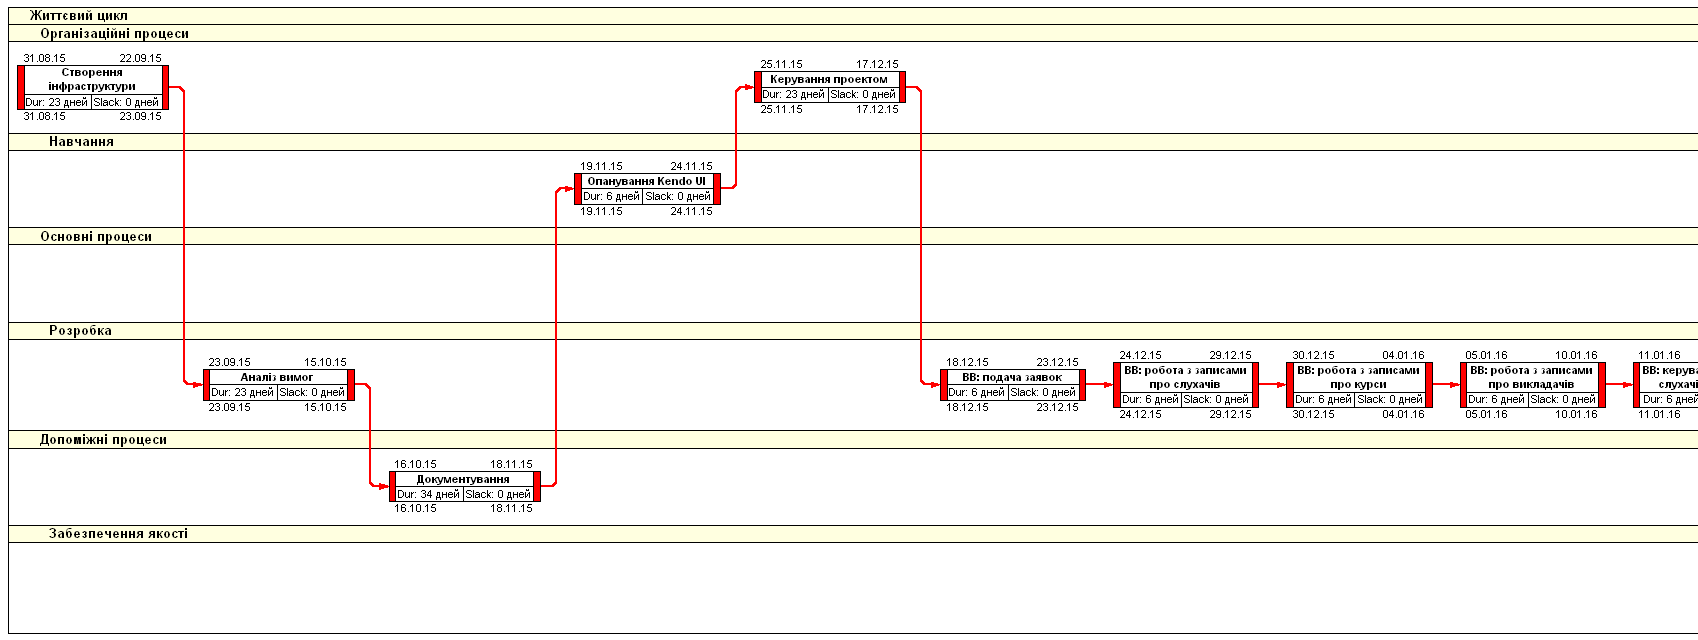
\includegraphics[width=24cm]{smp_cgw2_2.png}\\
\imglabel{Діаграма WBS}
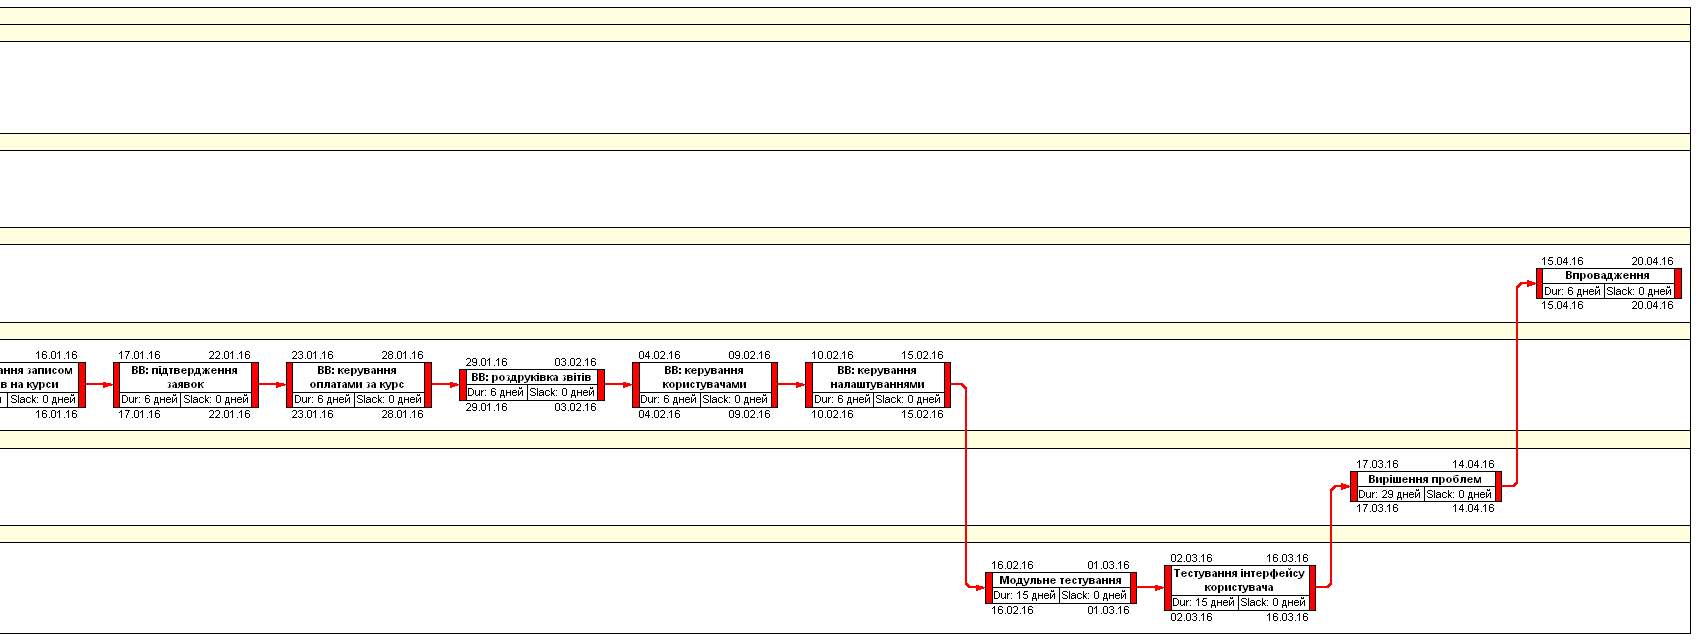
\includegraphics[width=24cm]{smp_cgw2_3.png}\\
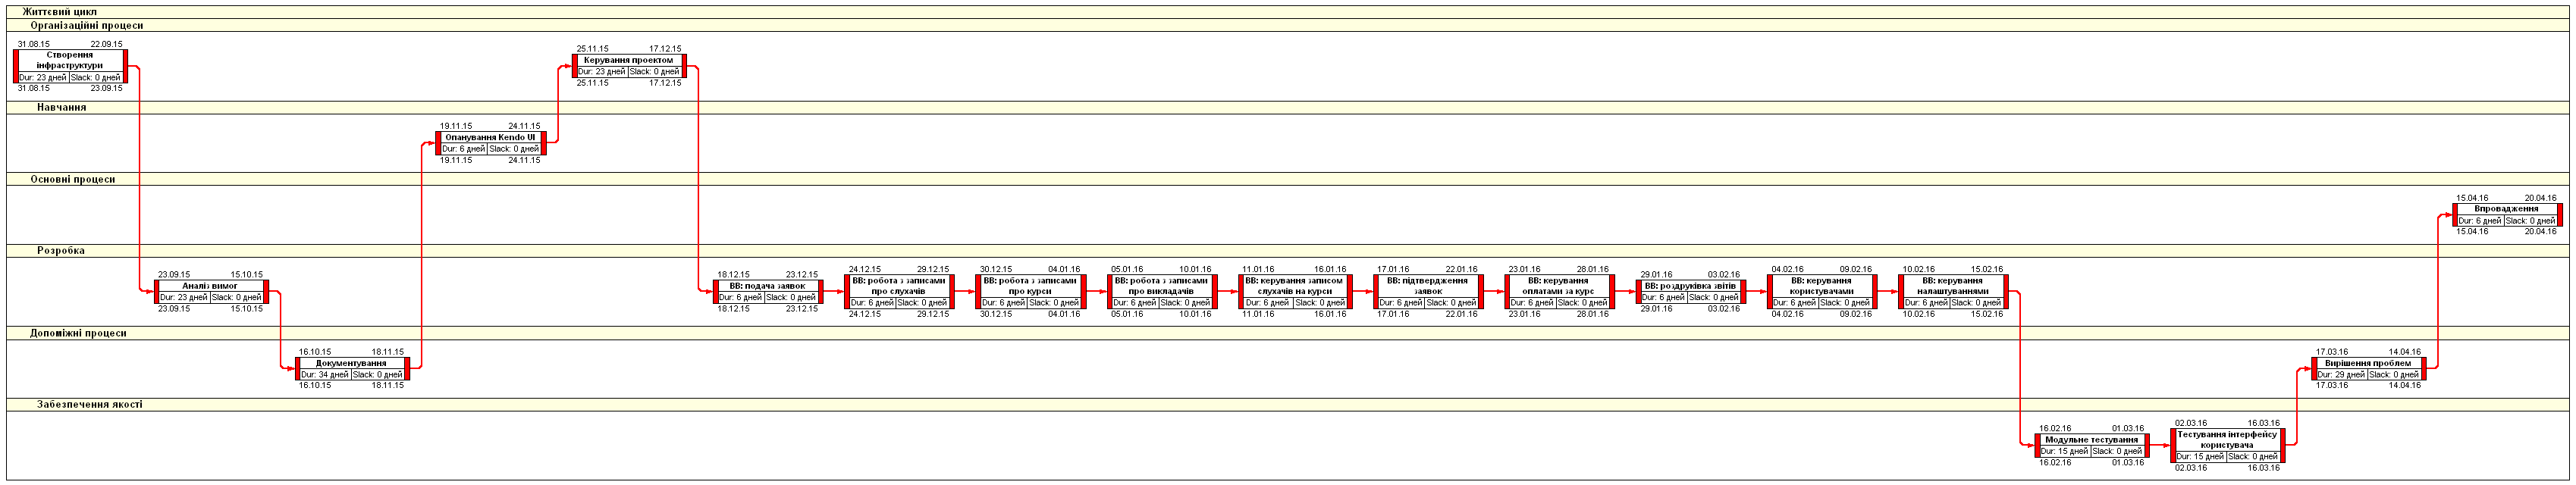
\includegraphics[width=24cm]{smp_cgw2_4.png}
\imglabel{Діаграма WBS (продовження)}
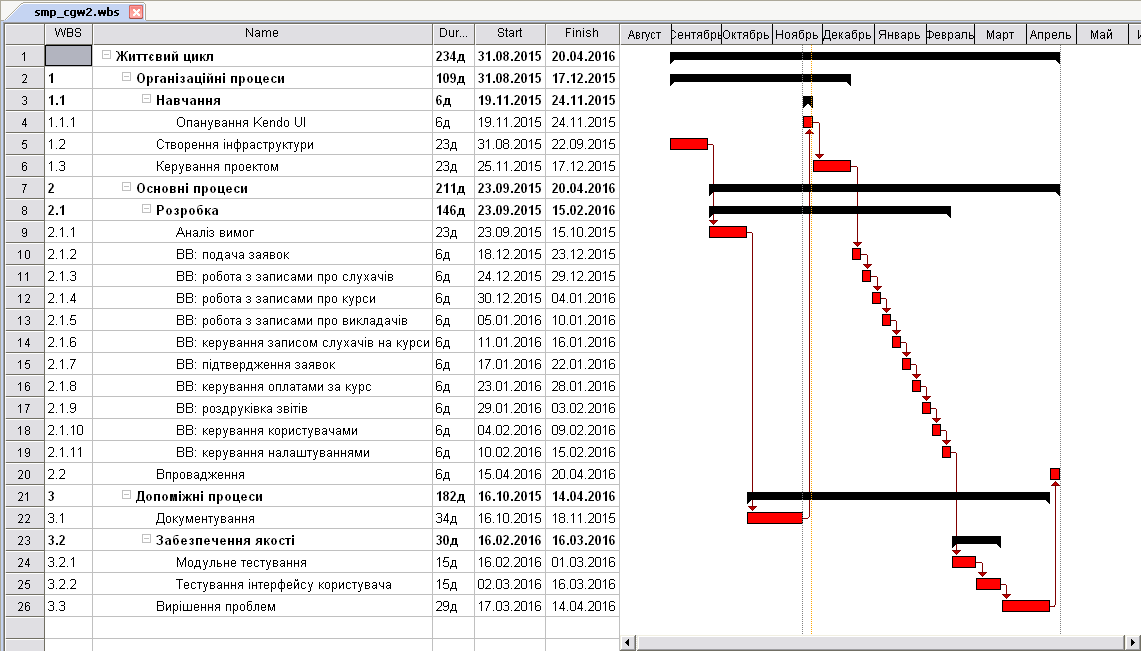
\includegraphics[width=24cm]{smp_cgw2_1.png}
\imglabel{Діаграма Ганта}
\end{landscape}

\bigbreak
\section{Проектування програмного продукту}
\subsection{Концептуальне проектування}
\bigbreak
Діаграму концептуальних класів наведено на рис. 6.

\noindent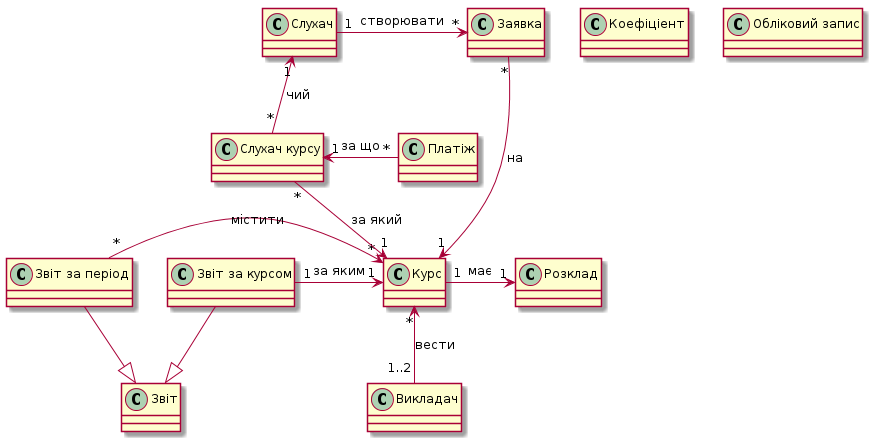
\includegraphics[width=17cm]{pp_pw3_conc.png}
\imglabel{Діаграма концептуальних класів}

Клас <<Курс>> характеризується високою зв'язністю, тобто це головний клас у системі.
\newpage
\subsection{Логічне проектування}
\bigbreak
Діаграму програмних класів наведено на рис. 7.

\noindent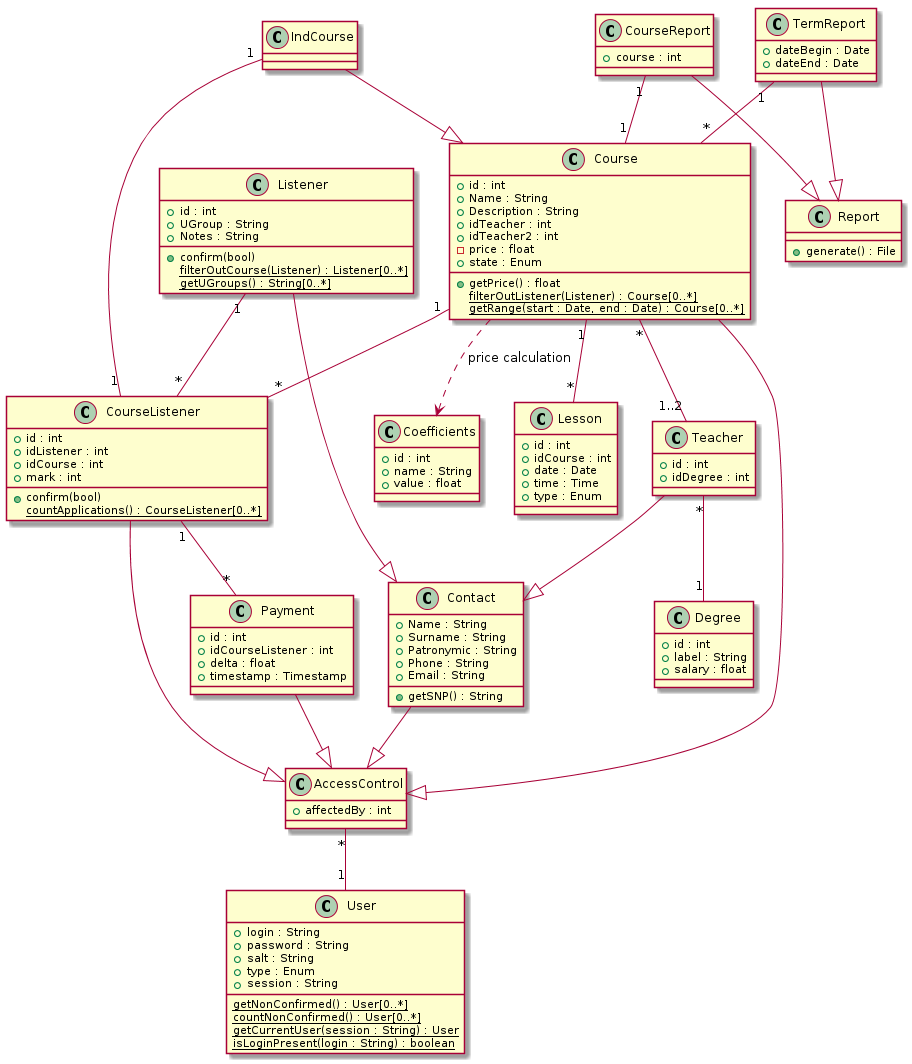
\includegraphics[width=17cm]{pp_pw3_clas.png}
\imglabel{Діаграма програмних класів}

Як і на діаграмі концептуальних класів, клас Course характеризується високою зв'язністю та має найбільшу кількість атрибутів. Також високу зв'язність має AccessControl, що відповідає висновку з пункту 1.2.1.

\newpage
\subsection{База даних}
\bigbreak
\def\dbhead{
 \hline
 \Centering Ключ &
 \Centering Назва &
 \Centering Ім'я поля &
 \Centering Тип &
 \Centering NULL &
 \Centering Дод.\\
 \hline
}
\tablefirsthead{\dbhead}
\tablelasttail{}
\tablehead{\hline \multicolumn{4}{|l|}{Продовження таблиці \thesection .\thetabcount} \\\dbhead}
\tabletail{\hline}
\def\dbtable#1#2#3{
 \tablabel{Опис структури таблиці "#1" (#2)}\\
 \begin{supertabular}{|p{1.2cm}|p{3.5cm}|p{3cm}|p{2.8cm}|p{1.2cm}|p{4.3cm}|}
 #3
 \hline
 \end{supertabular}
 \\[-3mm]
}
\newcommand{\tabheader}[2]{
 #1 \emph{(#2)}
}
\setlength{\tabcolsep}{3pt}
\dbtable{Слухачі}{listeners}{
PK & Ідентифікатор & idListener & int(6) & Ні & A\_I\\
 & Ім'я & Name & varchar(30) & Так & \\
 & Прізвіще & Surname & varchar(30) & Ні & \\
 & По батькові & Patronymic & varchar(30) & Так & \\
 & Університетська група & UGroup & varchar(6) & Так & \\
 & Телефон & Phone & varchar(20) & Так & \\
 & E-mail & Email & varchar(40) & Так & \\
FK & Ким змінено & affectedBy & varchar(32) & Ні & \\
}
\dbtable{Курси}{courses}{
PK & Ідентифікатор & idCourse & int(6) & Ні & A\_I\\
 & Назва & Name & varchar(50) & Ні & \\
 & Опис & Description & varchar(400) & Так & \\
 & Ознака індивідуального курсу & isIndividual & bit(1) & Ні & \\
FK & Викладач & idTeacher & int(6) & Так & \\
FK & Другий викладач & idTeacher2 & int(6) & Так & \\
 & Ціна & Price & decimal(10,2) & Так & \\
 & Стан & state & tinyint(1) & Ні & 0..2 (Йде набір, набрано, завершений)\\
FK & Ким змінено & affectedBy & varchar(32) & Ні & \\
}
\dbtable{Слухачі курсу}{Course\_Listeners}{
PK & Ідентифікатор & idCL & int(6) & Ні & A\_I\\
FK & Курс & idCourse & int(6) & Ні & \\
FK & Слухач & idListener & int(6) & Ні & \\
 & Оцінка & mark & tinyint(3) & Так & \\
FK & Ким змінено & affectedBy & varchar(32) & Ні & \\
}
\dbtable{Платежі}{payments}{
PK & Ідентифікатор & idPayment & int(6) & Ні & A\_I\\
FK & Слухач курсу & idCL & int(6) & Ні & \\
 & Кошти & delta & int(6) & Ні & \\
 & Мітка часу & timestamp & timestamp & Ні & CURRENT\_\ TIMESTAMP\\
}
\dbtable{Викладачі}{teachers}{
PK & Ідентифікатор & idTeacher & int(6) & Ні & A\_I\\
 & Ім'я & Name & varchar(30) & Так & \\
 & Прізвіще & Surname & varchar(30) & Ні & \\
 & По батькові & Patronymic & varchar(30) & Так & \\
 & Телефон & Phone & varchar(20) & Так & \\
 & E-mail & Email & varchar(40) & Так & \\
FK & Ким змінено & affectedBy & varchar(32) & Ні & \\
FK & Вчений ступінь & degree & tinyint(2) & Так & \\
}
\dbtable{Розцінки}{prices}{
PK & Ідентифікатор & degree & tinyint(2) & Ні & A\_I\\
 & Вчений ступінь & deglab & varchar(30) & Ні & \\
 & Зарплата & salary & decimal(10,2) & Ні & \\
}
\dbtable{Коефіціенти}{coefficients}{
PK & Назва & name & varchar(64) & Ні & \\
 & Мітка & label & varchar(128) & Так & \\
 & Значення & value & float & Так & \\
}
\newpage
\dbtable{Заняття}{lessons}{
PK & Ідентифікатор & idLesson & int(11) & Ні & A\_I\\
FK & Курс & idCourse & int(11) & Ні & \\
 & Дата & date & date & Так & \\
 & Час початку & time & time & Ні & \\
 & Тип & type & tinyint(1) & Ні & 0..1 (Лекція, Практика)\\
}
\dbtable{Користувачі}{users}{
PK & Логін & login & varchar(32) & Ні & \\
 & Хеш паролю & password & text & Ні & \\
 & Сіль & salt & text & Ні & \\
 & Тип & type & tinyint(1) & Ні & 0..2 (Оператор, Адміністратор, Переглядач)\\
 & Ключ сесії & sessionid & text & Так & \\
}
\bigbreak
\subsection{Оцінка алгоритмічної складності}
\bigbreak
\tikzset{
	line/.style={draw, -latex'},
	every join/.style={line},
	u/.style={anchor=south},
	r/.style={anchor=west},
	fxd/.style={text width = 6em},
	it/.style={font={\small\itshape}},
	bf/.style={font={\small\bfseries}}
}
\tikzstyle{base} =
	[
		draw,
		on chain,
		on grid,
		align=center,
		minimum height=4ex,
		minimum width = 10ex,
		node distance = 6mm and 60mm,
		text badly centered
	]
\tikzstyle{coord} =
	[
		coordinate,
		on chain,
		on grid
	]
\tikzstyle{cloud} =
	[
		base,
		ellipse,
		fill = red!5,
		node distance = 3cm,
		minimum height = 2em
	]
\tikzstyle{decision} =
	[
		base,
		diamond,
		aspect=2,
		fill = green!10,
		node distance = 2cm,
		inner sep = 0pt
	]
\tikzstyle{block} =
	[
		rectangle,
		base,
		fill = blue!3,
		rounded corners,
		minimum height = 2em
	]
\tikzstyle{print_block} =
	[
		base,
		tape,
		tape bend top=none,
		fill = yellow!10
	]
\tikzstyle{io} =
	[
		base,
		trapezium,
		trapezium left angle = 70,
		trapezium right angle = 110,
		fill = blue!5
	]
\makeatletter
\pgfkeys{/pgf/.cd,
	subrtshape w/.initial=2mm,
	cycleshape w/.initial=2mm
}
\pgfdeclareshape{subrtshape}{
	\inheritsavedanchors[from=rectangle]
	\inheritanchorborder[from=rectangle]
	\inheritanchor[from=rectangle]{north}
	\inheritanchor[from=rectangle]{center}
	\inheritanchor[from=rectangle]{west}
	\inheritanchor[from=rectangle]{east}
	\inheritanchor[from=rectangle]{mid}
	\inheritanchor[from=rectangle]{base}
	\inheritanchor[from=rectangle]{south}
	\backgroundpath{
		\southwest \pgf@xa=\pgf@x \pgf@ya=\pgf@y
		\northeast \pgf@xb=\pgf@x \pgf@yb=\pgf@y
		\pgfmathsetlength\pgfutil@tempdima{\pgfkeysvalueof{/pgf/subrtshape w}}
		\def\ppd@offset{\pgfpoint{\pgfutil@tempdima}{0ex}}
		\def\ppd@offsetm{\pgfpoint{-\pgfutil@tempdima}{0ex}}
		\pgfpathmoveto{\pgfqpoint{\pgf@xa}{\pgf@ya}}
		\pgfpathlineto{\pgfqpoint{\pgf@xb}{\pgf@ya}}
		\pgfpathlineto{\pgfqpoint{\pgf@xb}{\pgf@yb}}
		\pgfpathlineto{\pgfqpoint{\pgf@xa}{\pgf@yb}}
		\pgfpathclose
		\pgfpathmoveto{\pgfpointadd{\pgfpoint{\pgf@xa}{\pgf@yb}}{\ppd@offsetm}}
		\pgfpathlineto{\pgfpointadd{\pgfpoint{\pgf@xa}{\pgf@ya}}{\ppd@offsetm}}
		\pgfpathlineto{\pgfpointadd{\pgfpoint{\pgf@xb}{\pgf@ya}}{\ppd@offset}}
		\pgfpathlineto{\pgfpointadd{\pgfpoint{\pgf@xb}{\pgf@yb}}{\ppd@offset}}
		\pgfpathclose
	}
}
\pgfdeclareshape{cyclebegshape}{
	\inheritsavedanchors[from=rectangle]
	\inheritanchorborder[from=rectangle]
	\inheritanchor[from=rectangle]{north}
	\inheritanchor[from=rectangle]{center}
	\inheritanchor[from=rectangle]{west}
	\inheritanchor[from=rectangle]{east}
	\inheritanchor[from=rectangle]{mid}
	\inheritanchor[from=rectangle]{base}
	\inheritanchor[from=rectangle]{south}
	\backgroundpath{
		\southwest \pgf@xa=\pgf@x \pgf@ya=\pgf@y
		\northeast \pgf@xb=\pgf@x \pgf@yb=\pgf@y
		\pgfmathsetlength\pgfutil@tempdima{\pgfkeysvalueof{/pgf/cycleshape w}}
		\pgfpathmoveto{\pgfqpoint{\pgf@xa}{\pgf@ya}}
\pgfpathlineto{\pgfpointadd{\pgfpoint{\pgf@xa}{\pgf@yb}}{\pgfpoint{0ex}{-\pgfutil@tempdima}}}
\pgfpathlineto{\pgfpointadd{\pgfpoint{\pgf@xa}{\pgf@yb}}{\pgfpoint{\pgfutil@tempdima}{0ex}}}
\pgfpathlineto{\pgfpointadd{\pgfpoint{\pgf@xb}{\pgf@yb}}{\pgfpoint{-\pgfutil@tempdima}{0ex}}}
\pgfpathlineto{\pgfpointadd{\pgfpoint{\pgf@xb}{\pgf@yb}}{\pgfpoint{0ex}{-\pgfutil@tempdima}}}
\pgfpathlineto{\pgfqpoint{\pgf@xb}{\pgf@ya}}
		\pgfpathclose
	}
}
\pgfdeclareshape{cycleendshape}{
	\inheritsavedanchors[from=rectangle]
	\inheritanchorborder[from=rectangle]
	\inheritanchor[from=rectangle]{north}
	\inheritanchor[from=rectangle]{center}
	\inheritanchor[from=rectangle]{west}
	\inheritanchor[from=rectangle]{east}
	\inheritanchor[from=rectangle]{mid}
	\inheritanchor[from=rectangle]{base}
	\inheritanchor[from=rectangle]{south}
	\backgroundpath{
		\southwest \pgf@xa=\pgf@x \pgf@ya=\pgf@y
		\northeast \pgf@xb=\pgf@x \pgf@yb=\pgf@y
		\pgfmathsetlength\pgfutil@tempdima{\pgfkeysvalueof{/pgf/cycleshape w}}
		\pgfpathmoveto{\pgfqpoint{\pgf@xb}{\pgf@yb}}
\pgfpathlineto{\pgfpointadd{\pgfpoint{\pgf@xb}{\pgf@ya}}{\pgfpoint{0ex}{\pgfutil@tempdima}}}
\pgfpathlineto{\pgfpointadd{\pgfpoint{\pgf@xb}{\pgf@ya}}{\pgfpoint{-\pgfutil@tempdima}{0ex}}}
\pgfpathlineto{\pgfpointadd{\pgfpoint{\pgf@xa}{\pgf@ya}}{\pgfpoint{\pgfutil@tempdima}{0ex}}}
\pgfpathlineto{\pgfpointadd{\pgfpoint{\pgf@xa}{\pgf@ya}}{\pgfpoint{0ex}{\pgfutil@tempdima}}}
\pgfpathlineto{\pgfqpoint{\pgf@xa}{\pgf@yb}}
		\pgfpathclose
	}
}
\makeatother
\tikzstyle{subroutine} =
	[
		base,
		subrtshape,
		fill = green!25
	]
\tikzstyle{cyclebegin} =
	[
		base,
		cyclebegshape,
		fill = blue!25
	]
\tikzstyle{cycleend} =
	[
		base,
		cycleendshape,
		fill = blue!25
	]
\tikzstyle{connector} =
	[
		base,
		circle,
		fill = red!25,
		minimum width = 3mm
	]

На рис. 8 зазначено складну операцію розрахунку вартості за даними з БД. Вона реалізується наступним SQL-запитом:

\begin{figure}[t]
\begin{center}
{ \fontsize{12pt}{14pt} \selectfont
\begin{tikzpicture}[%
    start chain=going below,
    node distance=5mm and 60mm,
        ]
        \node [cloud] (start) {getCoursePrice(id, full)};
	\node [block, join] (global) {PRICE\_TRUNK := 10};
	\node [block, join] (q1) {price := вартість з таблиці courses\\для курсу id,};
	\node [decision, join] (q1cond) {price = 0};
	\node [block, join] (q2) {count := кількість слухачів\\з таблиці Course\_Listeners\\для курсу id};
	\node [block, join] (q3) {salary := (зарплата з таблиці prices\\для вченого ступеню з таблиці teachers\\для викладача з таблиці courses) *\\(кількість занять з таблиці lessons\\з типом <<Лекція>>) + (зарплата з таблиці prices\\для вченого ступеню з таблиці teachers\\для другого викладача з таблиці courses) *\\(кількість занять з таблиці lessons\\з типом <<Практика>>)};
        \node [subroutine, join, subrtshape w = 3mm, fxd] (coefficients) {coef := getCoefficients()};
	\node [block, join] (price) {price := $\left[ \frac{salary \cdot coef.personal \cdot coef.bonus \cdot coef.others}{count \cdot PRICE\_TRUNK}\right] \cdot PRICE\_TRUNK$};
	\node [decision, join] (fullcond) {full};
	\node [block] (fullmul) {price := $price \cdot count$};
        \node [cloud, join] (finish) {Повернення price};

        \path [line] (q1cond) to node [r] {Так} (q2);
        \path [line] (q1cond) -- node [u,near start] {Ні} ++(7cm, 0cm) |- (finish);
        \path [line] (fullcond) to node [r] {Так} (fullmul);
        \path [line] (fullcond) -- node [u,near start] {Ні} ++(3cm, 0cm) |- (finish);
\end{tikzpicture}
}
\end{center}
\imglabel{Алгоритм розрахунку вартості курсу}
\end{figure}

{ \fontsize{11pt}{12pt} \selectfont
\begin{verbatim}
SELECT ifnull(s1,0)*ifnull(c1,0)+ifnull(s2,0)*ifnull(c2,0) FROM ((
 SELECT salary as s1 FROM prices WHERE degree IN (
  SELECT degree FROM teachers WHERE idTeacher IN (
   SELECT idTeacher FROM courses WHERE idCourse=?
))) s1 LEFT OUTER JOIN (
 SELECT salary as s2 FROM prices WHERE degree IN(
  SELECT degree FROM teachers WHERE idTeacher IN (
   SELECT idTeacher2 FROM courses WHERE idCourse=63
))) s2 ON 1=1) LEFT OUTER JOIN ((
 SELECT count(*) as c1 FROM lessons WHERE idCourse=? AND type=0
) c1 ON 1=1 LEFT OUTER JOIN (
 SELECT count(*) as c2 FROM lessons WHERE idCourse=? AND type=1
) c2) ON 1=1;
\end{verbatim}
}

\FloatBarrier
План виконання запиту:
\begin{enumerate}
\item Вибірка вмісту таблиці courses
\item Проекція кортежів за значенням атрибуту idCourse
\item Проекція атрибутів за атрибутом idCourse
\item Вибірка вмісту таблиці teachers
\item Проекція кортежів за значенням атрибуту idTeacher
\item Проекція атрибутів за атрибутом degree
\item Вибірка вмісту таблиці prices
\item Проекція кортежів за значенням атрибуту degree
\item Проекція атрибутів за атрибутом salary
\item Використання вибірки з п. 1.
\item Проекція кортежів за значенням атрибуту idCourse
\item Проекція атрибутів за атрибутом idCourse
\item Використання вибірки з п. 4.
\item Проекція кортежів за значенням атрибуту idTeacher
\item Проекція атрибутів за атрибутом degree
\item Використання вибірки з п. 7.
\item Проекція кортежів за значенням атрибуту degree
\item Проекція атрибутів за атрибутом salary
\item Вибірка вмісту таблиці lessons
\item Проекція кортежів за значенням атрибуту idCourse
\item Проекція кортежів за значенням атрибуту type
\item Підрахунок кортежів
\item Використання проекції з п. 20.
\item Проекція кортежів за значенням атрибуту type
\item Підрахунок кортежів
\item З'єднання результатів пп. 9 та 18.
\item З'єднання результатів пп. 22 та 25.
\item З'єднання результатів пп. 26 та 27.
\item Розрахунок математичного виразу за результатом п. 28.
\end{enumerate}

Операції проекції кортежів у пп. 2, 3, 5, 6, 8, 9, 11, 12, 14, 15, 17 та 18 повинні повертати один кортеж. Пошук у таблицях courses та teachers відбувається за первинним ключем, а таблиця prices складається з кількох кортежів. Для проекцій з пп. 20, 21 та 24 доцільно створити у таблиці lessons індекс за атрибутом idCourse. За атрибутом type індекс недоцільний, оскільки проекції за ним відбуваються не з усієї таблиці, а можливих значення тільки два. SQL-запит для створення індексу:

{ \fontsize{11pt}{12pt} \selectfont
\begin{verbatim}
CREATE INDEX course_of_lesson ON lessons (idCourse);
\end{verbatim}
}

Циклів в алгоритмах на рис. 8 та 9 немає, тож їх складність --- O(N).

\begin{figure}[t]
\begin{center}
{ \fontsize{12pt}{14pt} \selectfont
\begin{tikzpicture}[%
    start chain=going below,
    node distance=5mm and 60mm,
        ]
        \node [cloud] (start) {user\_login(login, pass)};
	\node [block, join] (config) {config := з файлу конфігурації};
	\node [block, join] (q1) {user[password, salt, sessionid] := з\\таблиці users для логіну login};
	\node [decision, join] (q1cond) {user = $\emptyset$};
	\node [decision, yshift=-3mm] (confcond) {sessionid = <<q>>};
	\node [block] (crypt) {hash := crypt(pass,\\config.global\_salt)};
	\node [decision, join] (passcond) {pass = hash};
	\node [block] (gensess) {sess\_id := randhash(login, 500)};
	\node [block, join] (updsess) {Встановити в\\таблиці users\\sessionid := sess\_id\\для логіну login};
	\node [block, join] (cookiesess) {Записати sess\_id в Cookies};
	\node [block, join] (gotomain) {Перейти на головну сторінку};
        \node [cloud, join] (finish) {Вихід};

	\node [block, right of = q1cond, node distance = 8.5cm, yshift = -5mm] (err5) {Помилка 400:\\користувача не знайдено};
	\node [block, right of = confcond, node distance = 6.2cm, yshift = -5mm] (err10) {Помилка 403:\\обліковий запис\\ще не підтверджено};
	\node [block, right of = passcond, node distance = 4.5cm, yshift = -5mm] (err6) {Помилка 403:\\пароль невірний};

        \path [line] (q1cond) to node [r] {Ні} (confcond);
        \path [line] (q1cond) -| node [u,near start] {Так} (err5);
        \path [line] (err5) |- node {} (finish);
        \path [line] (confcond) to node [r] {Ні} (crypt);
        \path [line] (confcond) -| node [u,near start] {Так} (err10);
        \path [line] (err10) |- node {} (finish);
        \path [line] (passcond) to node [r] {Так} (gensess);
        \path [line] (passcond) -| node [u,near start] {Ні} (err6);
        \path [line] (err6) |- node {} (finish);
\end{tikzpicture}
}
\end{center}
\imglabel{Алгоритм аутентифікації та авторизації}
\end{figure}

\bigbreak
\subsection{Опис зовнішних інтерфейсів}
\bigbreak
Інтерфейс користувача побудовано із використанням бібліотеки Kendo UI, дизайн визначається наявними для неї темами оформлення. Доступні самостійні концептуальні класи присутні у головному меню та розташовані за частотою використання: найактивніша робота проводиться зі слухачами та курсами, викладачі та користувачі заповнюються на початку роботи і потім змінюються рідко, звіти здаються рідко, розцінки та коефіціенти змінюються у виключних випадках. В кінці головного меню розміщено кнопку виходу з системи. Екрану авторизації є окремим та лаконічним, містить лише форму та кнопку перемикання форм реєстрації та входу.

Для роботи серверної частини системи потрібен веб-сервер Apache 2.x, інтерпретатор PHP5 не нижче 5.4, СКБД MySQL або MariaDB 5. Для користування клієнтською частиною потрібен web-браузер із підтримкою EcmaScript 5; тестування проводиться у поточних версіях браузерів Mozilla Firefox та Chromium для десктопу.

Система може працювати у межах однієї машини, через локальну мережу та через мережу Інтернет, в залежності від мережевих підключень та налаштувань машини, на якій встановлено серверну частину. Підключення, відповідно, може здійснюватись будь-яким доступним дротовим або бездротовим каналом підключення до локальної мережі або мережі Інтернет: Ethernet, Wi-Fi, ADSL, HSPA, Dial-up та ін. Оскільки звіти генеруються у форматі PDF, для їх перегляду потрібна програма --- переглядач PDF: Mozilla Firefox, Google Chrome, Adobe Reader, Foxit Reader тощо. Для друку потрібен принтер, підключений безпосередньо до машини, на якій відкрито файл звіту, або доступний для неї через мережу.
\FloatBarrier

\newpage
\section{Конструювання програмного продукту}
\subsection{Опис програмних технологій}
\bigbreak
Система поділяється на дві частини: сервер та клієнт.

Сервер реалізовано на мові PHP5. [11] Це скриптова мова програмування, орієнтована на задачі web-розробки. Завдяки відсутності етапу компіляції зменшується час розробки та відлагодження. Динамічна типізація мови дозволяє прозоро працювати як з числами, так і з їх текстовим представленням, а також спрощує перевірку наявності об'єктів у булевих виразах. Мова надає вбудовані засоби для обробки рядків, параметрів HTTP-запитів та взаємодії з різними СКБД. Окрім цього, PHP є єдиною підтримуваною мовою на багатьох хостингах для web-сайтів та web-застосунків. З цієї ж причини у якості СКБД обрано MySQL 5. Задля використання нових можливостей, зокрема, скороченого оголошення масивів, мінімальною підтримуваною версією є PHP 5.4.

Клієнт реалізовано на скриптовій мові програмування ECMAScript 5 (більше відомій як JavaScript) та описових мовах HTML 5 та CSS 3. Вони є фактичними web-стандартами та підтримуються сучасними web-браузерами, такими як Firefox, Chrome, Edge, Safari, Internet Explorer, Android Browser тощо. Альтернативи не є кросбраузерними, приміром, мова VBScript підтримується лише у Internet Explorer, а мова Dart --- лише у Chrome. Крім того, використання web-технологій дозволяє створювати на основі клієнту застосунки для настільних та мобільних комп'ютерів за допомогою спеціальних середовищ на основі браузерних рушіїв (напр., node-webkit, PhoneGap, AppJS).
\bigbreak
\subsection{Опис програмних бібліотек}
\bigbreak
Оскільки клієнт є <<товстим>>, на сервер покладені лише задачі передачі та обробки даних між клієнтом та базою даних, тож немає потреби у використанні систем керування контентом, фреймворків та тому подібних бібліотек. Проте мова PHP не має вбудованих засобів для побудови PDF-документів, тож для цієї задачі використано бібліотеку MPDF, яка формує документ з HTML-шаблону. Серед альтернатив розглядалася також бібліотеку TCPDF, проте при спробі використання вона виявила недостатню підтримку можливостей HTML та CSS.

Модульні тести для сервеу також написані мовою PHP та використовують бібліотеку Dogpatch, розширену та доповнену для потреб тестування системи. Бібліотека DogPatch дозволяє виконувати HTTP-запити та таким чином перевіряти, чи вірні відповіді та HTTP-коди надають запити за певних умов. Додано функції для обробки відповідей у JSON, що дозволяють перевірити наявність певного об'єкту у масиві об'єктів.

Клієнт використовує бібліотеки jQuery та Kendo UI. jQuery є прошарком над API, що доступні для браузерного JavaScript, який надає компактний синтаксис та кросбраузерні реалізації для таких частовживаних операцій, як робота з DOM та AJAX-запитами. Kendo UI надає елементи керування (віджети) із широкою фукціональністю, у тому числі такі, що не надаються засобами HTML. Крім того, вона надає багатофункціональний елемент керування для представлення та редагування табличних даних, а також самостійно здійснює запити з цими даними до серверу, слід лише описати URL та формати даних. [12] Для призначення гарячих клавіш використовується плаґін для jQuery jquery.hotkeys.
\bigbreak
\subsection{Особливості створення програмних модулів з урахуванням мови програмування}
\bigbreak
\begin{sloppy}
Інтерпретатор та мова PHP5 розраховані на використання у якості CGI, тобто web-сервер використовує URI як відносний шлях до файлу, запускає файл на виконання та віддає результат його роботи. Альтернативні способи використання URI, зокрема, маскування структури програмних модулів за допомогою так званих <<людинозрозумілих URL>> та маршрутизації запитів до викликів методів класів вимагають низькорівневих перехоплень за допомогою правил ModRewrite для Apache та аналогічних засобів для інших web-серверів. Тому натомість архітектуру серверної частини системи реалізовано без застосування об'єктно-орієнтованого програмування, проте із наслідуванням деяких його принципів. Модулі організовані по директоріях за концептуальними класами і реалізують інтерфейси шляхом розміщення у директоріях файлів з однаковими іменами, способами передачі параметрів та форматами вхідних та вихідних даних --- це дозволяє за реалізації роботи з різними концептуальними класами у клієнті змінювати лише назву директорії. Функції для зв'язку між концептуальними класами винесено в окремі модулі, спільні функції винисено в окремі бібліотеки функцій.

Клієнт реалізовано як односторінковий застосунок. Головний інтерфейс системи реалізований HTML-сторінкою з меню; за натисненням пунктів меню створюються та відкриваються певні вікна засобами JavaScript. Проте сторінка входу та реєстрації, як незалежна від головного інтерфейсу сутність, винесена в окрему HTML-сторінку, до якої не підключено JavaScript-бібліотек. Обидві сторінки можуть змінюватисься в залежності від режиму, повідомлень системи, прав доступу тощо, тому виводяться скриптами на мові PHP, що є HTML-шаблонами зі вставками коду на PHP. Власних функцій на JavaScript небагато і слугують вони здебільшого прошарком між описами даних та реалізованими засобами бібліотеки Kendo UI елементами керування, тож зібрані в один модуль. За розвитку системи та додання нових функцій може знадобитися декомпозиція цього модулю.
\end{sloppy}
\bigbreak
\subsection{Особливості створення структур даних}
\bigbreak
У якості формату передачі даних від сервера до клієнту обрано JSON. Це текстовий формат на основі мови JavaScript, що надає компактний безнадлишковий (порівняно з похідними від SGML мовами) синтаксис та дозволяє структурувати рядки та числа у вкладених масивах та об'єктах (асоціативних масивах). [13] JSON формується засобами мови PHP, що доступні з версії 5.1. Дані від клієнта до сервера передаються у тілі POST-запиту у форматі HTML-форм. Структури даних, що використовуються при роботі з бібліотекою Kendo UI, визначаються документацією до цієї бібліотеки.

\bigbreak
\subsection{Модульне тестування}
\bigbreak
\tablabel{Тестові дані для таблиці courses}
\begin{center}
\begin{tabular}{|l|c|c|}
\hline
Атрибут & \multicolumn{2}{c|}{Значення} \\
\hline
idCourse & 1 & 2 \\
Name & a & b \\
Description & a & b \\
isIndividual & 0 & 0 \\
idTeacher & 1 & 1 \\
idTeacher2 & 2 & 2 \\
Price & 15 & 0 \\
state & 0 & 0 \\
affectedBy & user1 & user2 \\
\hline
\end{tabular}
\end{center}

\newpage
\tablabel{Тестові дані для таблиці Course\_Listeners}
\begin{center}
\begin{tabular}{|l|c|c|c|c|}
\hline
Атрибут & \multicolumn{4}{c|}{Значення} \\
\hline
idCL & 1 & 2 & 3 & 4 \\
idCourse & 1 & 1 & 1 & 2 \\
idListener & 1 & 2 & 3 & 1 \\
mark & 0 & 0 & 0 & 0 \\
affectedBy & user1 & user1 & user1 & user1 \\
\hline
\end{tabular}
\end{center}

\tablabel{Тестові дані для таблиці teachers}
\begin{center}
\begin{tabular}{|l|c|c|}
\hline
Атрибут & \multicolumn{2}{c|}{Значення} \\
\hline
idTeacher & 1 & 2 \\
Name & a & b \\
Surname & a & b \\
Patronymic & a & b \\
Phone & 289 & 2893 \\
Email & b@a.b & c@d.c \\
degree & 1 & 2 \\
affectedBy & user1 & user2 \\
\hline
\end{tabular}
\end{center}

\tablabel{Тестові дані для таблиці prices}
\begin{center}
\begin{tabular}{|l|c|c|c|}
\hline
Атрибут & \multicolumn{3}{c|}{Значення} \\
\hline
degree & 1 & 2 & 3 \\
deglab & Б. с. & Доц. к. т. н. & Проф. \\
salary & 15.62 & 23.24 & 35.38 \\
\hline
\end{tabular}
\end{center}

\tablabel{Тестові дані для таблиці lessons}
\begin{center}
\begin{tabular}{|l|c|c|c|c|c|c|}
\hline
Атрибут & \multicolumn{6}{c|}{Значення} \\
\hline
idLesson & 1 & 2 & 3 & 4 & 5 & 6 \\
idCourse & 1 & 1 & 1 & 2 & 2 & 2 \\
date & 1.4.15 & 2.4.15 & 3.4.15 & 4.4.15 & 5.4.15 & 6.4.15 \\
time & 13:00 & 13:00 & 13:00 & 13:00 & 13:00 & 13:00 \\
type & 1 & 1 & 2 & 1 & 2 & 2 \\
\hline
\end{tabular}
\end{center}

\newpage
\tablabel{Тестові дані для таблиці users}
\begin{center}
\begin{tabular}{|l|c|c|c|}
\hline
Атрибут & \multicolumn{3}{c|}{Значення} \\
\hline
login & adm1 & user1 & user2 \\
password & $hash('asdf')$ & $hash('qwer')$ & $hash('zxcv')$ \\
salt & $<hash1>$ & $<hash2>$ & $<hash3>$ \\
type & 0 & 1 & 2 \\
sessionid & $<key1>$ & NULL & q \\
\hline
\end{tabular}
\end{center}

{\setlength{\tabcolsep}{0pt}
\tablabel{Тестові дані для таблиці coefficients}
\begin{center}
\begin{tabular}{|l|c|c|c|}
\hline
Атрибут & \multicolumn{3}{c|}{Значення} \\
\hline
name & bonus & others & personal \\
label & \parbox{4.5cm}{Нарахування на заробітну плату} & Інші послуги та утримки & Зарплата персоналу \\
value & 1.12 & 1.23 & 1.05 \\
\hline
\end{tabular}
\end{center}}

Тестування алгоритму розрахунку вартості курсу проведено методом "білої скрині" (таблиця 3.7), алгоритму аутентифікації та авторизації --- методом "чорної скрині" (таблиця 3.8).
\tablabel{Тестові випадки для алгоритму розрахунку вартості курсу}
\newcounter{tcnt}\def\tcn{\addtocounter{tcnt}{1} \thetcnt}
\begin{tabular}{|c|c|c|c|c|}
\hline
\multirow{2}{23mm}{\centering \textbf{Test Case №}} &
\multicolumn{2}{c|}{\textbf{Вхідні дані}} &
\multirow{2}{27mm}{\centering \textbf{Очікуваний результат}} &
\multirow{2}{77mm}{\centering \textbf{Результат тестування (успішний (passed) / неуспішний (failed))}} \tabularnewline
\cline{2-3}
&id&full&&\tabularnewline
\hline
\tcn& 1	& true	& 60	&	\\
\tcn& 2	& true	& 15	&	\\
\tcn& 1	& false	& 20	&	\\
\tcn& 2	& false	& 15	&	\\
\hline
\end{tabular}
\setcounter{tcnt}{0}
\tablabel{Тестові випадки для алгоритму аутентифікації та авторизації}\\
\begin{tabular}{|c|c|c|c|c|}
\hline
\multirow{2}{18mm}{\centering \textbf{Test Case №}} &
\multicolumn{2}{c|}{\textbf{Вхідні дані}} &
\multirow{2}{27mm}{\centering \textbf{Очікуваний результат}} &
\multirow{2}{75mm}{\centering \textbf{Результат тестування (успішний (passed) / неуспішний (failed))}} \tabularnewline
\cline{2-3}
&login&pass&&\tabularnewline
\hline
\tcn& 'adm1'	& 'asdf'	& Вхід		&	\\
\tcn& 'adm1'	& 'qwer'	& Відмова	&	\\
\tcn& 'adm1'	& NULL		& Відмова	&	\\
\tcn& 'user3'	& 'qwer'	& Відмова	&	\\
\tcn& 'user3'	& 'sdfj'	& Відмова	&	\\
\tcn& 'user2'	& 'zxcv'	& Відмова	&	\\
\hline
\end{tabular}

%\newcounter{tcnt}\def\tcn{\addtocounter{tcnt}{1} \thetcnt}
\setcounter{tcnt}{0}
\def\testhead{
 \hline
 \Centering \textbf{Test Case №} &
 \Centering \textbf{Дія} &
 \Centering \textbf{Очікуваний результат} &
 \Centering \textbf{Результат тестування} \\\hline
}
\tablefirsthead{\testhead}
\tablelasttail{}
\tablehead{\hline \multicolumn{4}{|l|}{Продовження таблиці \thesection .\thetabcount} \\\testhead}
\tabletail{\hline}
%
\addtolength{\textheight}{-2cm}
\bigbreak
\subsection{Функціональне тестування}
\bigbreak
Проведено функціональне тестування, сценарій для якого створено на основі основних та альтернативних сценаріїв варіантів використання (табл. 3.10)
\tablabel{Тестові випадки для варіантів використання}\\[-\baselineskip]
\nopagebreak[4]
\begin{center}
\begin{supertabular}{|p{11mm}|p{70mm}|p{55mm}|p{3cm}|}
\tcn
& Перейти на сторінку реєстрації
& Відкрилася сторінка реєстрації
& Passed
\\ \hline \tcn
& Ввести логін test111 та двічі --- пароль test111
& Повідомлення про успішну реєстрацію
& Passed
\\ \hline \tcn
& Ввести логін test222 та двічі --- пароль test222
& Повідомлення про успішну реєстрацію
& Passed
\\ \hline \tcn
& Перейти на сторінку входу
& Відкрилася сторінка входу
& Passed
\\ \hline \tcn
& Ввести логін asdf та пароль asdf
& Система відхилює авторизацію
& Passed
\\ \hline \tcn
& Ввести логін test111 та пароль test111
& Система відхилює авторизацію
& Passed
\\ \hline \tcn
& Ввести логін asdf та пароль adsf
& Відкрився головний інтерфейс системи (рядок меню)
& Passed
\\ \hline \tcn
& Відкрити таблицю викладачів
& З'явилася таблиця
& Passed
\\ \hline \tcn
& Створити викладача (<<Ппшш>> <<Шррр>> <<Тссс>> <<+3820>> <<ba@b.c>>), зберегти зміни та оновити список
& Викладач присутній в списку та дані не пошкоджено
& Passed
\\ \hline \tcn
& Змінити ім'я щойно створеного викладача на <<Шссс>>, зберегти зміни та оновити список
& Ім'я викладача змінилося, дані не пошкоджено
& Passed
\\ \hline \tcn
& Відкрити таблицю курсів
& З'явилася таблиця
& Passed
\\ \hline \tcn
& Створити курс (<<>> <<Шррр>> <<Ппшш Ш. Т.>> <<29>> <<Йде набір>>) та зберегти зміни
& Система вимагає ввести назву курсу
& Passed
\\ \hline \tcn
& Створити курс (<<Ппшш>> <<Шррр>> <<Ппшш Ш. Т.>> <<Ппшш Ш. Т.>> <<29>> <<Йде набір>>), зберегти зміни та оновити список
& Курс присутній в списку та дані не пошкоджено
& Passed
\\ \hline \tcn
& Змінити назву щойно створеного курсу на <<Ппрр>>, зберегти зміни та оновити список
& Назва курсу змінилася, дані не пошкоджено
& Passed
\\ \hline \tcn
& Відкрити для щойно створеного курсу форму додання заняття
& Відкрилася форма
& Passed
\\ \hline \tcn
& Створити для щойно створеного курсу заняття (<<01.04.2016>> <<13:30>> <<Лекція>>), зберегти зміни та оновити список
& Заняття присутнє в списку та дані не пошкоджено
& Passed
\\ \hline \tcn
& Змінити час щойно створеного заняття на <<13:45>>, зберегти зміни та оновити список
& Час змінився, дані не пошкоджено
& Passed
\\ \hline \tcn
& Створити для щойно створеного курсу заняття (<<02.04.2016>> <<13:30>> <<Практика>>), зберегти зміни та оновити список
& Заняття присутнє в списку та дані не пошкоджено
& Passed
\\ \hline \tcn
& Видалити заняття за дату 01.04.2016 та оновити список
& Заняття відсутнє у списку
& Passed
\\ \hline \tcn
& Встановити для заняття, що залишилося, тип <<Лекція>>, зберегти зміни та оновити список
& Тип змінився, дані не пошкоджено
& Passed
\\ \hline \tcn
& Відкрити таблицю слухачів
& З'явилася таблиця
& Passed
\\ \hline \tcn
& Створити слухача (<<Шшпп>> <<Ршшш>> <<Сттт>> <<АЯ-313>> <<+3289>> <<db@d.b>> <<>>), зберегти зміни та оновити список
& Слухач присутній в списку та дані не пошкоджено
& Passed
\\ \hline \tcn
& Змінити ім'я щойно створеного слухача на <<Ртдм>>, зберегти зміни та оновити список
& Ім'я слухача змінилося, дані не пошкоджено
& Passed
\\ \hline \tcn
& Розгорнути для щойно створеного слухача підтаблицю запису на курси
& Розгорнулася підтаблиця
& Passed
\\ \hline \tcn
& Записати слухача на курс <<Ппрр>>
& Курс з'явився в підтаблиці
& Passed
\\ \hline \tcn
& Перейти в таблицю <<Курси>>
& Таблиця перекрила інші таблиці
& Passed
\\ \hline \tcn
& Розгорнути для курсу <<Ппрр>> підтаблицю слухачів
& Підтаблиця розгорнулася і містить слухача <<Шшпп Р. С.>>
& Passed
\\ \hline \tcn
& Встановити слухачеві <<Шшпп Р. С.>> оплату <<29>>, зберегти зміни та оновити список
& Оплата 29 грн., боргу немає
& Passed
\\ \hline \tcn
& Відкрити форму створення звіту за період
& Відкрилася форма
& Passed
\\ \hline \tcn
& Обрати дати 29.02.2016 та 28.02.2016 і створити звіт
& Система не приймає дати
& Passed
\\ \hline \tcn
& Обрати дати 29.02.2037 та 01.03.2037 і створити звіт
& Система не приймає дати
& Passed
\\ \hline \tcn
& Обрати дати 01.04.2016 та 02.04.2016 і створити звіт
& Відкривається або завантажується PDF-файл, що містить дані, відповідні даним у таблицях інтерфейсу
& Passed
\\ \hline \tcn
& Видалити заняття для курсу <<Ппрр>>
& Курс <<Ппрр>> не містить занять
& Passed
\\ \hline \tcn
& Видалити курс <<Ппрр>>, зберегти зміни та оновити список
& Курс відсутній у списку
& Passed
\\ \hline \tcn
& Перейти в таблицю <<Викладачі>>, видалити викладача Ппшш Шссс Тссс, зберегти зміни та оновити список
& Викладач відсутній у списку
& Passed
\\ \hline \tcn
& Створити у зовнішній системі три заявки, при цьому третю --- на ПІБ <<Шшпу Ртдм Стут>>, та зачекати 20 секунд
& Лічильник сповіщень збільшився на 3
& Passed
\\ \hline \tcn
& Відкрити сповіщення
& Відображається панель зі сповіщеннями
& Passed
\\ \hline \tcn
& Підтвердити реєстрацію облікового запису test111
& Сповіщення зникло зі списку
& Passed
\\ \hline \tcn
& Відхилити реєстрацію облікового запису test222
& Сповіщення зникло зі списку
& Passed
\\ \hline \tcn
& Підтвердити першу щойно додану заявку та перейти до таблиці <<Слухачі>>
& Сповіщення зникло зі списку сповіщень, слухач із заявки з'явився в таблиці
& Passed
\\ \hline \tcn
& Відхилити другу щойно додану заявку та оновити таблицю <<Слухачі>>
& Сповіщення зникло зі списку сповіщень та не з'явилося в таблиці
& Passed
\\ \hline \tcn
& Злити третю щойно додану заявку з запропонованим <<Шшпп Ртдм Сттт>>, обравши ПІБ із заявки, та оновити таблицю <<Слухачі>>
& Слухач відображається в таблиці з новим ПІБ
& Passed
\\ \hline \tcn
& Перейти в таблицю <<Слухачі>>, видалити слухача Шшпу Ртдм Стут, зберегти зміни та оновити список
& Слухач відсутній у списку
& Passed
\\ \hline \tcn
& Відкрити таблицю коефіціентів
& З'явилася таблиця
& Passed
\\ \hline \tcn
& Запам'ятати значення коефіціенту зарплати персоналу, встановити його у 1.3, зберегти зміни та оновити таблицю
& Коефіціент змінився, дані не пошкоджено
& Passed
\\ \hline \tcn
& Відновити значення коефіціенту зарплати персоналу, зберегти зміни та оновити таблицю
& Коефіціент змінився, дані не пошкоджено
& Passed
\\ \hline \tcn
& Вийти з системи
& Відкрився екран входу
& Passed
\\ \hline \tcn
& Увійти з логіном test111 та паролем test111
& Відобразилося меню системи
& Passed
\\ \hline \tcn
& Вийти з системи, увійти з логіном asdf та паролем adsf, відкрити таблицю користувачів
& З'явилася таблиця
& Passed
\\ \hline \tcn
& Скинути пароль для користувача test111, вийти з системи, увійти з логіном test111 та паролем test222
& Відобразилося меню системи
& Passed
\\ \hline \tcn
& Вийти з системи, увійти з логіном asdf та паролем adsf, відкрити таблицю користувачів, видалити користувача test111, зберегти зміни та оновити таблицю
& Користувач test111 зник зі списку
& Passed
\\ \hline \tcn
& Вийти з системи, увійти з логіном test111 та паролем test222
& Система відхилює авторизацію
& Passed
\\ \hline \tcn
& Увійти з логіном test222 та паролем test222
& Система відхилює авторизацію
& Passed
\\ \hline
\end{supertabular}
\end{center}
\addtolength{\textheight}{2cm}

\bigbreak
\section{Розгортання програмного продукту}
\subsection{Інструкція з встановлення}
\bigbreak
\begin{sloppy}
\begin{enumerate}
\item Встановити та налаштувати web-сервер Apache, інтерпретатор PHP5 не нижче версії 5.4, СКБД MySQL 5 або MariaDB 5. Для запуску сервера та клієнта на одній машині можна скористатися XAMPP з \url{https://www.apachefriends.org/ru/index.html}.
\item Скачати та розпакувати архів: \url{https://github.com/bodqhrohro/knp2014/archive/master.zip}.
\item Розпакувати вміст каталогу src з архіву до каталогу сторінок сайту. за необхідності налаштувати домен.
\item Встановити PHPMyAdmin (\url{https://www.phpmyadmin.net/}), перейти на вкладку "Імпорт" та вибрати файл deploy.sql з каталогу src. Впевнитися, що операція імпорту пройшла успішно.
\item Відкрити у текстовому редакторі файл config.php з кореневого каталогу сайту та вказати там IP чи домен СКБД, логін та пароль для доступу до БД, а також домен, на якому розміщено сайт. Зберегти файл.
\item Відкрити домен, на якому розміщено сайт, у браузері. Впевнитися, що відображається форма входу.\\
\includegraphics[width=17cm]{scrns/login.png}\imglabel{Форма входу}
\end{enumerate}
\end{sloppy}
\bigbreak
\subsection{Інструкція з використання}
\bigbreak
Демонстраційну копію системи розміщено на \url{http://php-bodqhrohro.rhcloud.com/knp2014/}.

В щойно встановленій системі є чотири тестових користувачі: адміністратор asdf, оператор fdsa, переглядачі pnd та qwer. Паролі для них, відповідно: adsf, fdsa, pnd, qwer. Можна запрошувати створення нових користувачів. Натисніть кнопку "Реєстрація" у верхньому правому кутку. введіть логін нового користувача та пароль. Підтвердіть форму, перейдіть знов на сторінку входу та спробуйте увійти під користувачем asdf. Відкриється головний інтерфейс системи --- стрічка меню.
\\
\includegraphics[width=17cm]{scrns/menu.png}\imglabel{Головне меню}

При реєстрації нового користувача адміністратори отримують сповіщення. Відкрийте з головного меню панель сповіщень та ввімкніть режим "Детально".
\begin{center}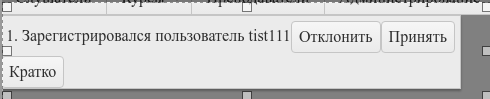
\includegraphics[width=10cm]{scrns/notifications.png}\end{center}\imglabel{Сповіщення}

Можна підтвердити користувача, після чого під ним можна буде зайти, або видалити його. Таким же чином оброблюються заявки слухачів на запис на курси. Щоб сховати панель, натисніть пункт "Сповіщення" ще раз.

Пункт "Вихід" головного меню викликає завершення сесії користувача та перехід на екран входу. Підменю "Звіти" містить пункти, що відкривають форми налаштування звітів. Решта пунктів відкривають таблиці. Натисніть, приміром, пункт "Слухачі". Відкриється таблиця для роботи зі слухачами.

Можна додавати нові рядки за допомогою кнопки на панелі інструментів, видаляти їх за допомогою кнопки зправа та редагувати, клацнувши на потрібній комірці. Змінені комірки підсвічуються. Всі зміни в таблиці не синхронізуються із сервером автоматично --- для цього слугує кнопка "Зберегти зміни". Якщо вміст якоїсь комірки перешкоджає збереженню, вона залишиться підсвіченою.

Таблиці "Слухачі" та "Курси" мають у кожному рядку підтаблиці, що дозволяють записувати слухачів на курси та працювати з оплатами. Розгортаються підтаблиці клацанням по трикутнику з лівого краю рядка. У підтаблицях не можна безпосередньо редагувати комірки, оплата вводиться у формі, що викликається кнопкою "Змінити". При поверненні грошей слухачеві вводиться від'ємна оплата. Додаються слухачі або групи з випадаючого списку; для слухачів він представлений у вигляді дерева з прапорцями, що дозволяє зручно додавати на курс цілі університетські групи та шукати слухачів за групами замість довгого алфавітного списку чи форми пошуку. Слухачі не з університету або з невідомої групи відображаються у піддереві "Інші".

Коли треба згенерувати звіт, виберіть потрібний звіт з випадаючого меню. За необхідності введіть діапазон дат та натисніть кнопку "Створити звіт". Якщо звіт не відкривається у браузері, його можна зберегти та відкрити будь-яким переглядачем PDF та з нього ж відправити на друк.

\bigskip
\section*{Висновки}
\bigskip
У даній дипломній роботі поставлено і вирішено завдання розробки системи обліку платних курсів із підтримкою самостійного запису слухачів через мережу Інтернет.

Експериментальним шляхом встановлено, що час, який витрачає асистент на реєстрацію слухача вручну, становить близько 5 хвилин. За використання системи реєстрація займає 4 хвилини, а за умови самостійного попереднього запису --- менше хвилини. Таким чином скорочується черга слухачів під час набору слухачів на курс, а час асистентів звільняється для інших видів робочої діяльності.

В першому розділі <<Визначення бізнес-вимог>> дипломної роботи приведені вимоги бізнес-рівня, функціональні, не функціональні, середовища функціонування, кваліфікація користувачів, проведений аналіз існуючих аналогів, з виділенням  переваг і недоліків.

В другому розділі <<Проектування програмного продукту>> описано проектування архітектури системи, структури та організації класів та бази даних.

В третьому розділі <<Конструювання програмного продукту>> представлені набір інструментальних засобів розробки та алгоритм програми, тестування функціональності системи та приклад її використання.

В четвертому розділі <<Розгортання програмного продукту>> наведено інструкції з встановлення та використання системи.

\def\biblitem#1#2#3{\item \sloppypar#1 [Електронний ресурс]. --- Режим доступу: URL: \url{#2}. --- #3.}
\newpage
\section*{Список використаних джерел}
\addcontentsline{toc}{section}{Список використаних джерел}
\bigskip
\begin{enumerate}
\biblitem{Автоматизація документообігу (обліку)}{http://erp-project.com.ua/index.php/uk/korisni-materiali/statti/avtomatizatsiya/339-avtomatizatsiya-dokumentoobigu-obliku}{1С ХАРКІВ ПРОЕКТ}
\biblitem{1С: Предприятие 8}{v8.1c.ru/}{1С: Предприятие 8}
\biblitem{Платформа}{http://www.parus.com/products/system/platform/}{Корпорация ПАРУС}
\biblitem{Внутренний портал учебного заведения}{http://www.1c-bitrix.ru/solutions/edu/university/}{1С-Битрикс}
\biblitem{Features}{https://docs.moodle.org/30/en/Features}{MoodleDocs}
\biblitem{Справка по Access - Служба поддержки Office}{https://support.office.com/ru-ru/article/Справка-по-Access-29d7b83c-3b06-41ca-b38b-483b6d5efb1b}{Справка и обучение по Microsoft Office --- поддержка Office}
\biblitem{Система приоритетов MoSCoW - Product management}{http://aclebedev.ru/moscow-method/}{Product management - Наблюдения, мысли и опыт управления продуктом в IT}
\biblitem{Зв'язність (програмування)}{https://uk.wikipedia.org/wiki/Зв'язність_(програмування)}{Вікіпедія}
\biblitem{Оценка программ}{http://www.structur.h1.ru/ocenka.htm}{Структуры и алгоритмы}
\biblitem{Бесплатные программы для просмотра PDF}{http://biblprog.org.ua/ru/pdf/}{BIBLPROG}
\biblitem{PHP Manual}{http://php.net/manual/en/index.php}{PHP: Hypertext Processor}
\biblitem{Kendo UI HTML Framework}{http://www.telerik.com/kendo-ui}{Telerik}
\biblitem{JSON: The Fat-Free Alternative to XML}{http://www.json.org/xml.html}{JSON}
\end{enumerate}

\newpage
\section*{Додаток А. Ілюстрації}
\setlength{\parindent}{0cm}
\addcontentsline{toc}{section}{Додаток А. Ілюстрації}
\begin{tikzpicture}
\makeatletter
\tikzset{
 circle connection bar/.style={rectangle,draw=\tikz@concept@color,every circle connection bar},
 every concept/.append style={minimum size=0cm, color=black, fill=white},
 concept/.style={circle,draw=\tikz@concept@color,every concept},
 every node/.append style={concept}
} \makeatother
\path[
 mindmap,
 scale=0.8,
 level 1 concept/.append style={sibling angle=120},
 level 2 concept/.append style={sibling angle=60},
 level 3 concept/.append style={sibling angle=30},
 level 4 concept/.append style={sibling angle=32,text width=1cm},
 sys/.style={concept, font=\footnotesize},
]
node [sys] {Система обліку платних курсів\\із підтримкою самостійного запису слухачів через мережу Інтернет} [clockwise from=210]
 child {
  node {Вхідний потік} [clockwise from=330]
   child { node {Хто?} [clockwise from=340]
    child { node {Оператори} }
    child { node [text width=1.4cm] {Адміністратор} }
    child [sibling angle=32] { node {Слухачі} [clockwise from=330]
     child { node {Студенти} }
     child { node {Сторонні} }
    }
   }
   child { node {Що?} [clockwise from=320]
    child { node {Дані слухачів} }
    child { node {Курси} }
    child { node {Дані викладачів} }
    child { node [text width=1.2cm] {Коефіціенти} }
    child { node {Розклад курсів} }
   }
   child { node {Де?} [clockwise from=200]
    child { node {Web-сайт} }
    child { node {Кафедра СПЗ} }
   }
   child { node {Коли?}  [clockwise from=180]
    child { node {Початок чверті} }
    child { node {Довільно} }
   }
   child { node {Як?} [clockwise from=150]
    child { node {Ручне введення} }
    child [sibling angle=45] { node {Імпорт з системи електронного деканату} }
   }
 } child {
  node [text width=2.5cm]{Внутрішній потік} [clockwise from=210]
   child { node {Хто?} }
   child { node {Що?} 
    child { node [text width=1.2cm] {Збереження даних} }
    child { node {Контроль цілісності} }
    child { node [text width=1.2cm] {Розрахунок вартості курсу} }
   }
   child { node {Де?} [clockwise from=105]
    child { node {Web-сервер} }
    child { node {СКБД} }
   }
   child { node {Коли?} [clockwise from=60]
    child { node {Постійно} }
   }
   child { node {Як?} [clockwise from=30]
    child { node {Формула} }
   }
 } child {
  node {Вихідний потік} [clockwise from=90]
   child { node {Хто?} [clockwise from=120]
    child { node {Викладачі} }
    child { node {Оператори} }
    child { node [text width=1.4cm] {Адміністратор} }
    child { node {Слухачі} [clockwise from=30]
     child { node {Студенти} }
     child { node {Сторонні} }
    }
   }
   child { node {Що?} [clockwise from=35]
    child { node [text width=1.2cm] {Сповіщення} }
    child { node {Звіти} 
     child { node {За період} }
     child { node {За курсом} }
    }
    child { node {Розклад} }
   }
   child { node {Де?} [clockwise from=10]
    child { node {Web-сайт} }
    child { node {Кафедра СПЗ} }
    child { node [text width=1.2cm] {Бухгалтерія} }
   }
   child { node {Коли?} [clockwise from=340]
    child { node {Кінець семестру} }
    child { node {Під час курсів} }
   }
   child { node {Як?} [clockwise from=300]
    child { node {Звіти} [clockwise from=320]
     child { node {У файл} }
     child { node {Друк} }
    }
    child { node [text width=1.2cm] {Сповіщення} [clockwise from=280]
     child { node {На e-mail} }
     child [sibling angle=40] { node {На сайті} }
    }
   }
 };
\end{tikzpicture}
\addimglabel{А}{Мозкова карта}
\newpage
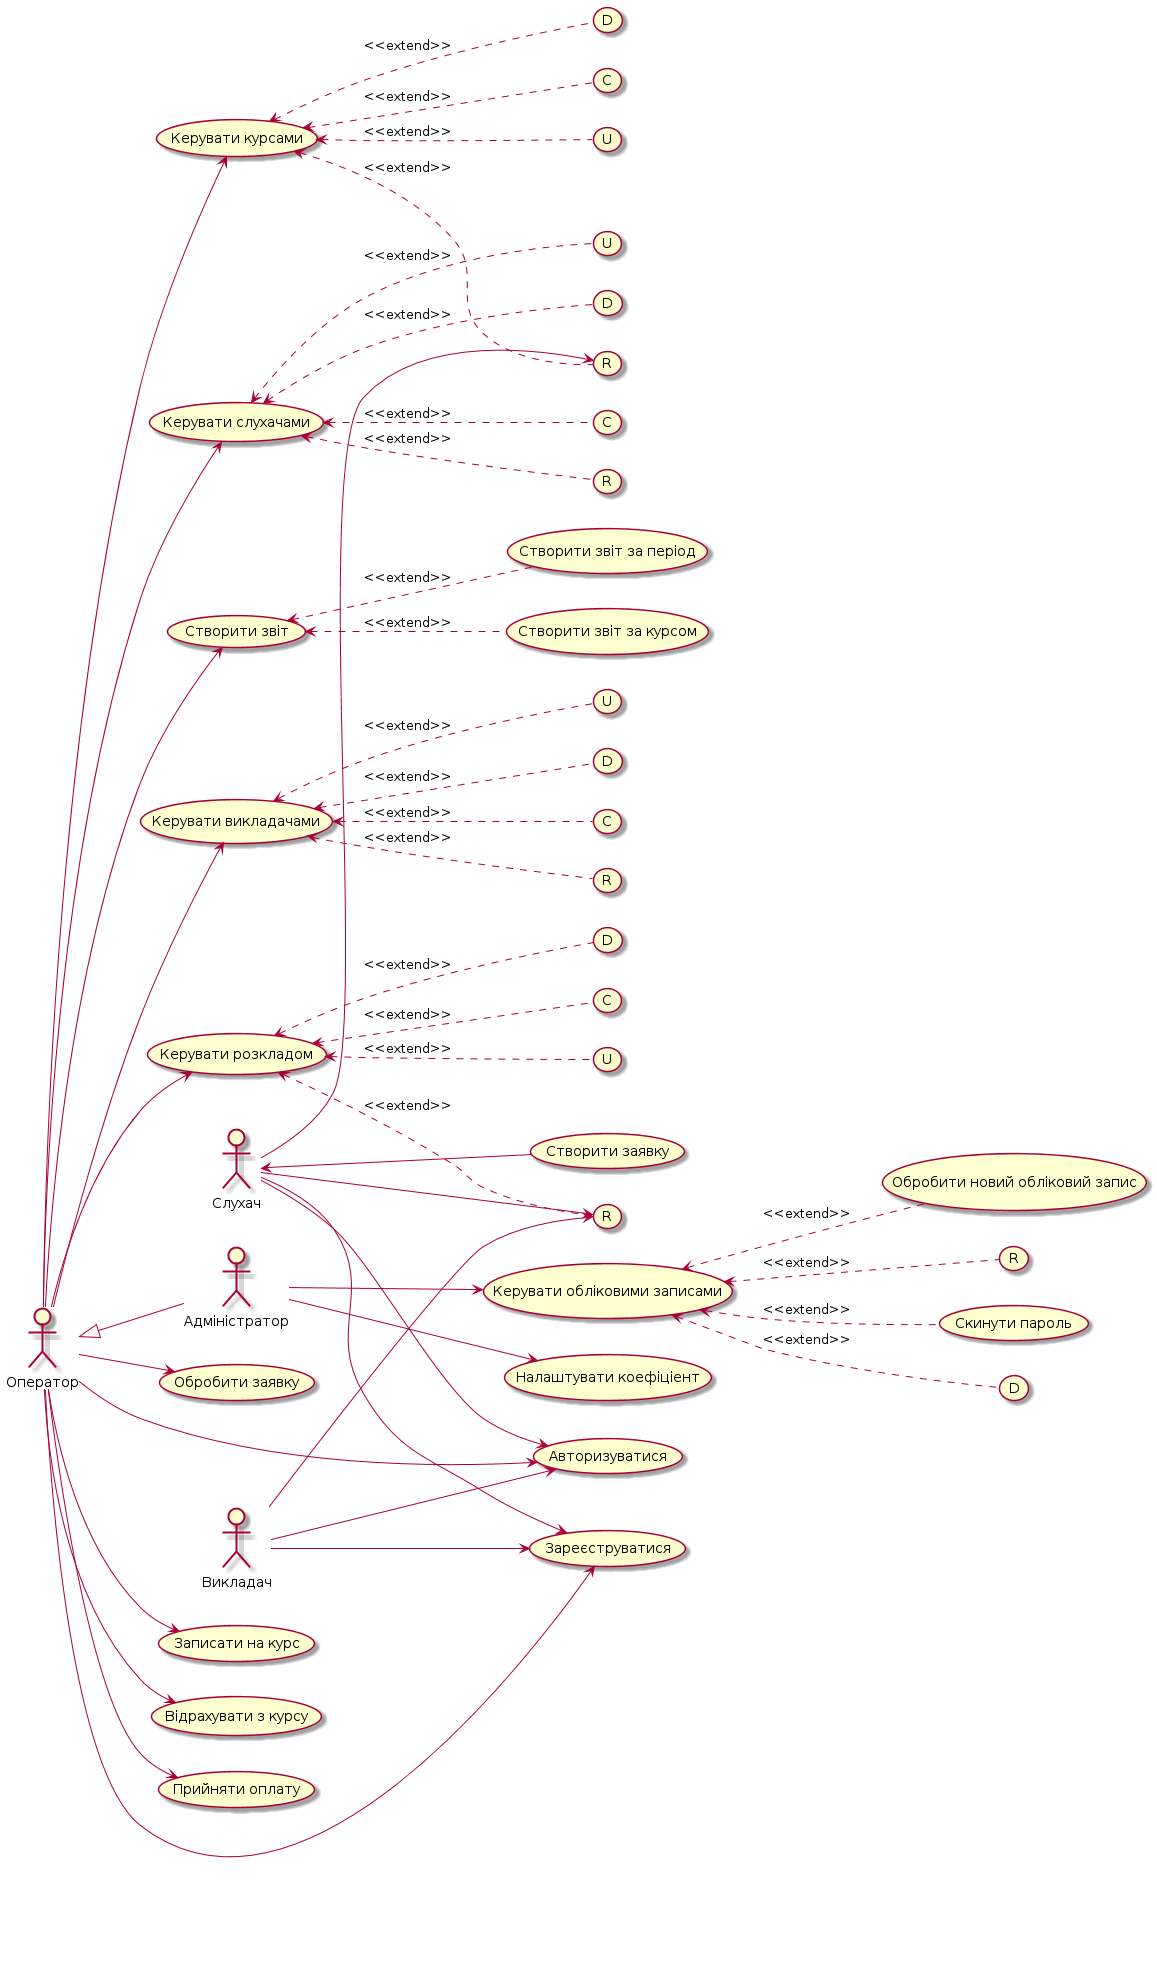
\includegraphics[width=14cm]{pp_pw1_uc.png}
\addimglabel{А}{Діаграма варіантів використання}

\begin{landscape}
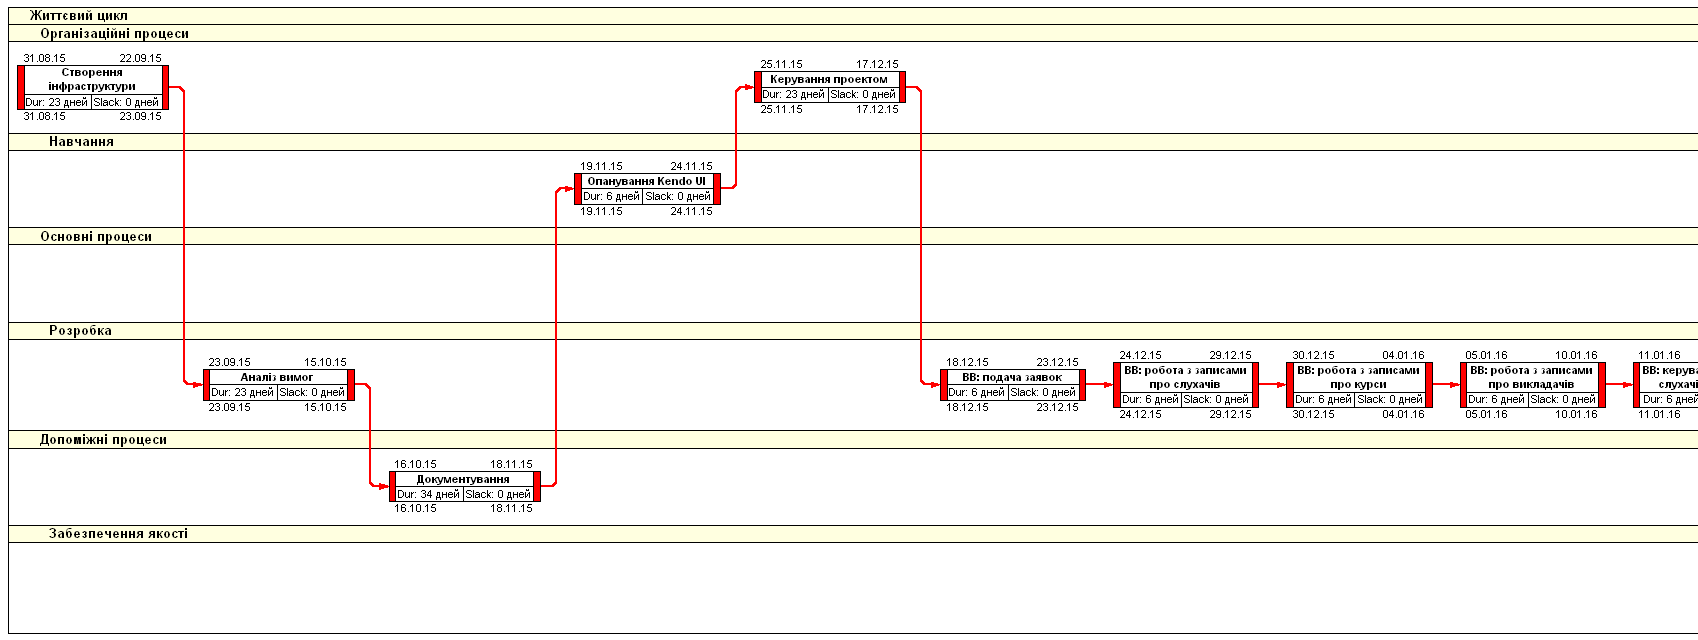
\includegraphics[width=24cm]{smp_cgw2_2.png}\\
\addpolyimglabel{А}{Діаграма WBS}{1}
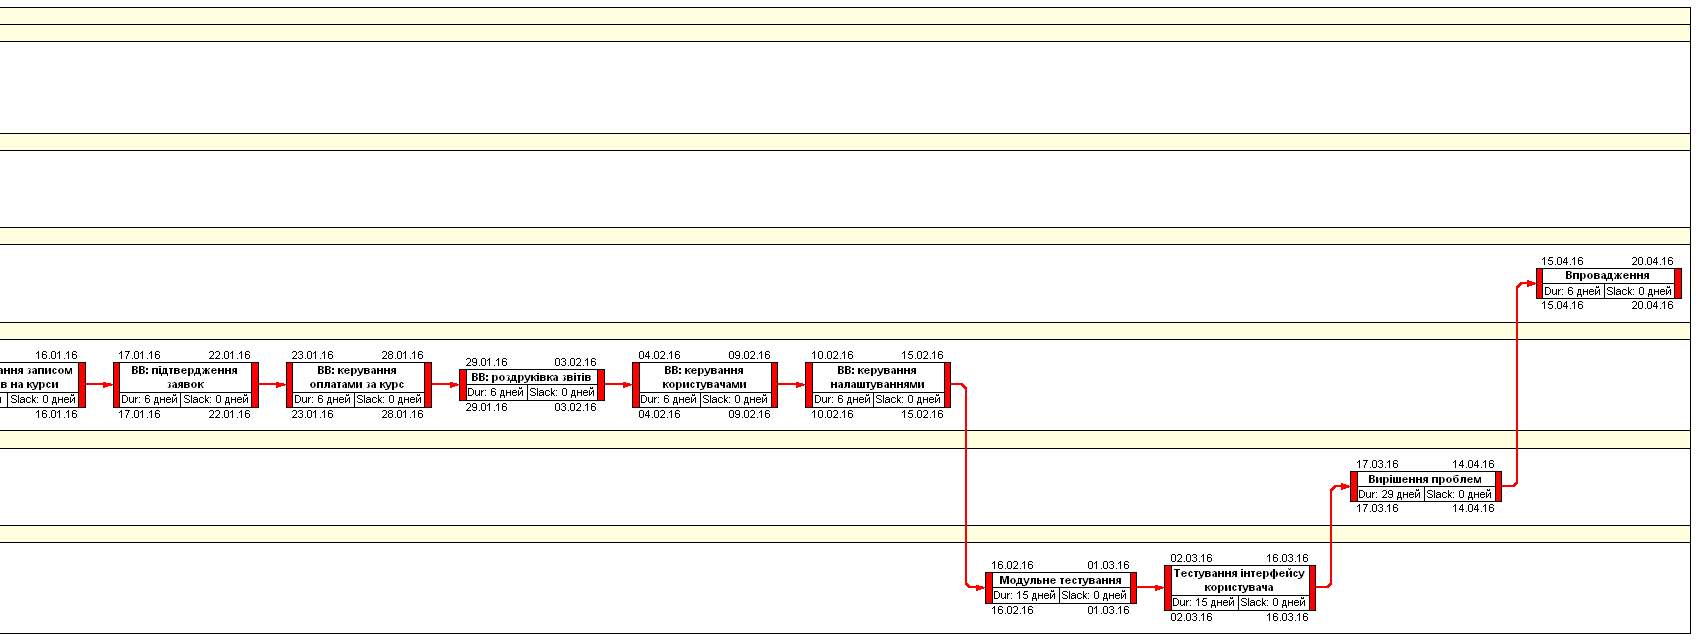
\includegraphics[width=24cm]{smp_cgw2_3.png}\\
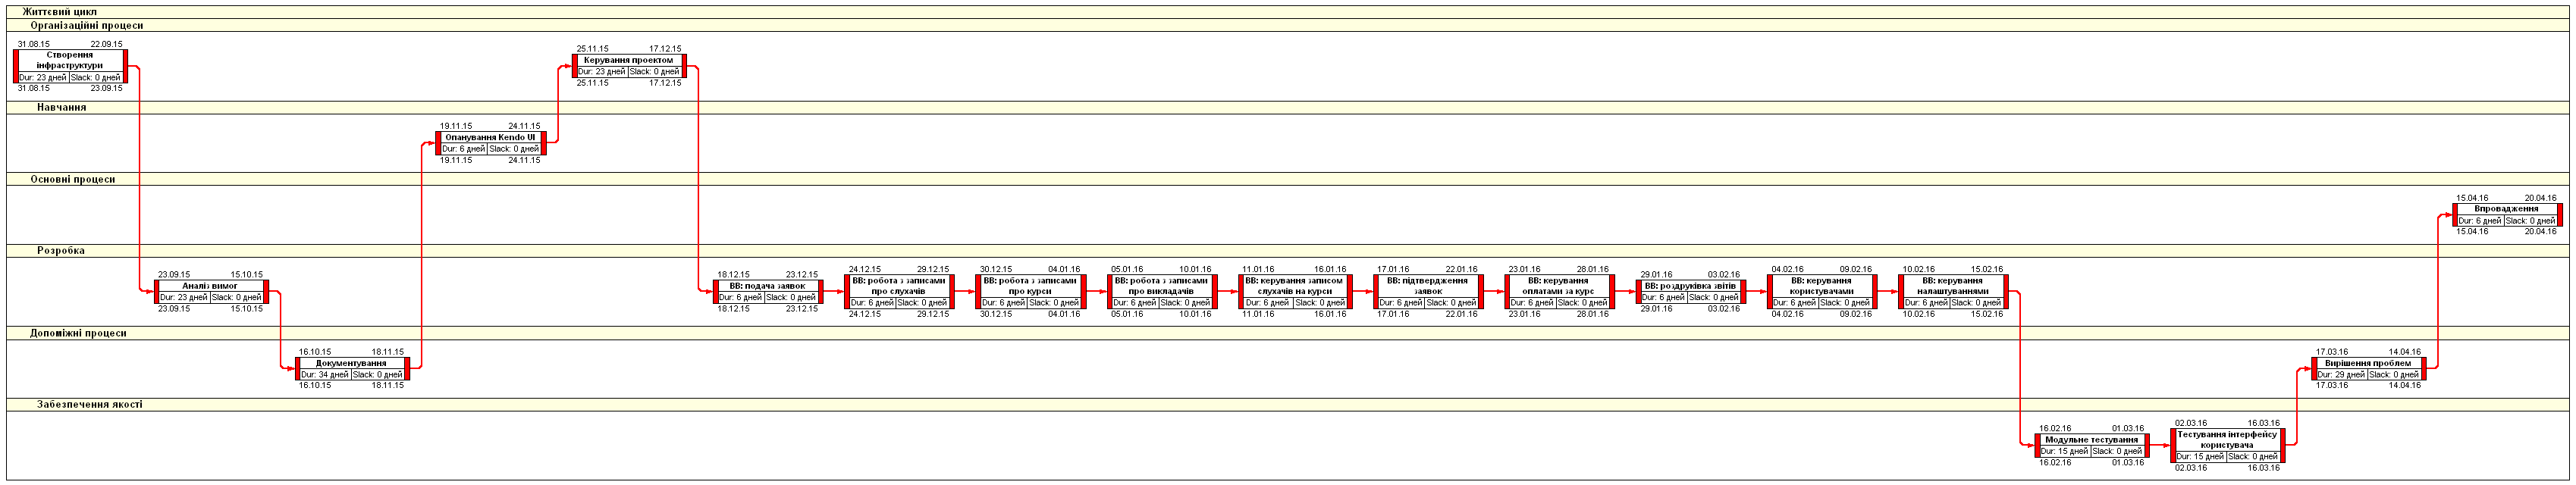
\includegraphics[width=24cm]{smp_cgw2_4.png}
\addtocounter{imgcount}{-1}
\addpolyimglabel{А}{Діаграма WBS}{2}
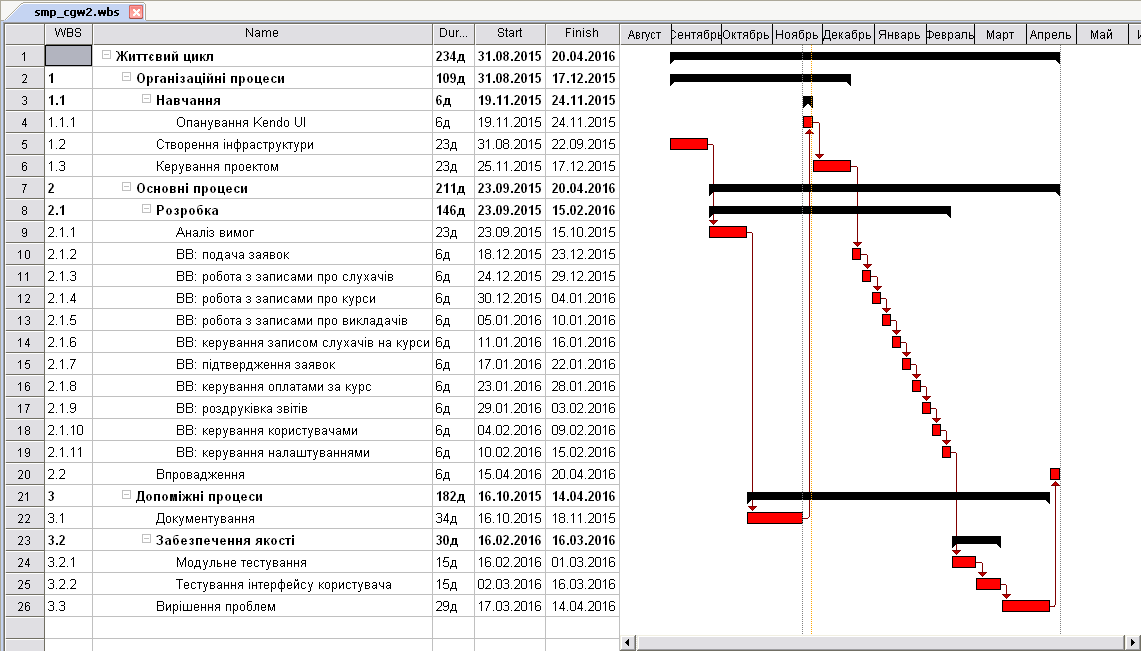
\includegraphics[width=24cm]{smp_cgw2_1.png}
\addimglabel{А}{Діаграма Ганта}
\end{landscape}

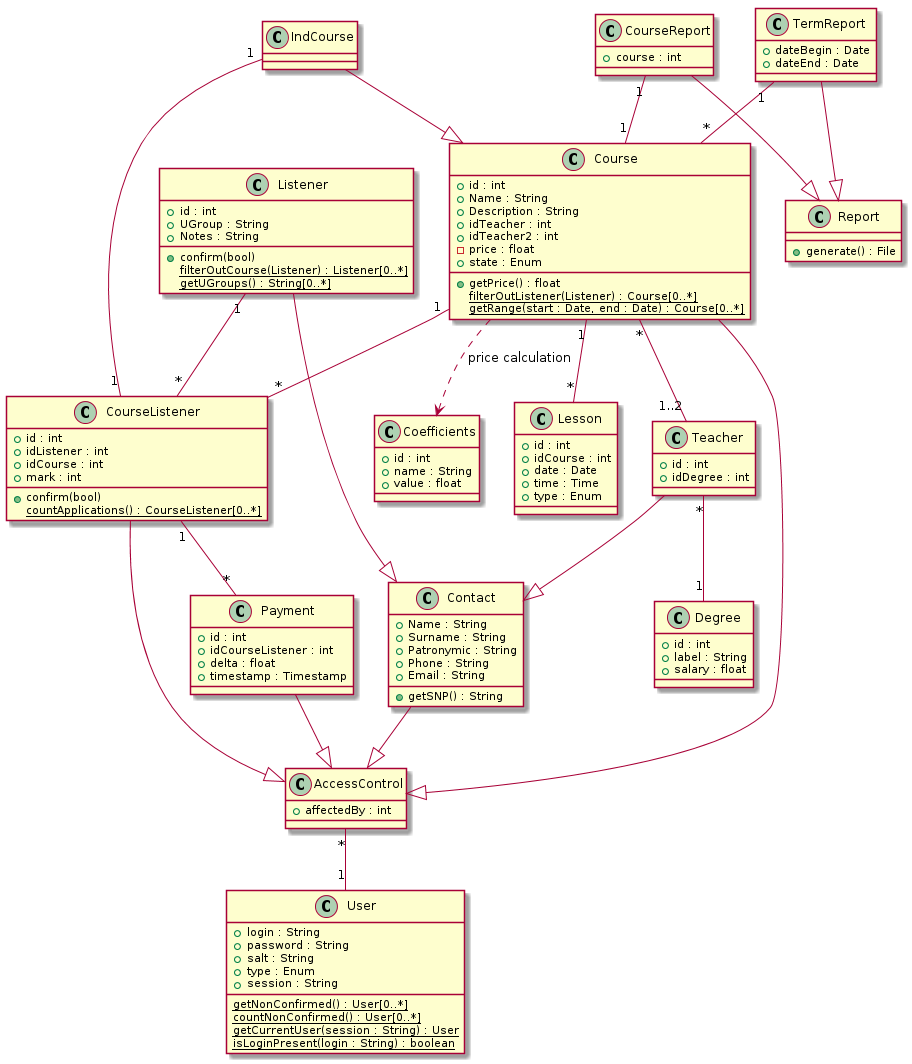
\includegraphics[width=17cm]{pp_pw3_clas.png}
\addimglabel{А}{Діаграма програмних класів}

\newpage
\tikzset{
	line/.style={draw, -latex'},
	every join/.style={line},
	u/.style={anchor=south},
	r/.style={anchor=west},
	fxd/.style={text width = 6em},
	it/.style={font={\small\itshape}},
	bf/.style={font={\small\bfseries}}
}
\tikzstyle{base} =
	[
		draw,
		on chain,
		on grid,
		align=center,
		minimum height=4ex,
		minimum width = 10ex,
		node distance = 6mm and 60mm,
		text badly centered
	]
\tikzstyle{coord} =
	[
		coordinate,
		on chain,
		on grid
	]
\tikzstyle{cloud} =
	[
		base,
		ellipse,
		fill = red!5,
		node distance = 3cm,
		minimum height = 2em
	]
\tikzstyle{decision} =
	[
		base,
		diamond,
		aspect=2,
		fill = green!10,
		node distance = 2cm,
		inner sep = 0pt
	]
\tikzstyle{block} =
	[
		rectangle,
		base,
		fill = blue!3,
		rounded corners,
		minimum height = 2em
	]
\tikzstyle{print_block} =
	[
		base,
		tape,
		tape bend top=none,
		fill = yellow!10
	]
\tikzstyle{io} =
	[
		base,
		trapezium,
		trapezium left angle = 70,
		trapezium right angle = 110,
		fill = blue!5
	]
\makeatletter
\pgfkeys{/pgf/.cd,
	subrtshape w/.initial=2mm,
	cycleshape w/.initial=2mm
}
\pgfdeclareshape{subrtshape}{
	\inheritsavedanchors[from=rectangle]
	\inheritanchorborder[from=rectangle]
	\inheritanchor[from=rectangle]{north}
	\inheritanchor[from=rectangle]{center}
	\inheritanchor[from=rectangle]{west}
	\inheritanchor[from=rectangle]{east}
	\inheritanchor[from=rectangle]{mid}
	\inheritanchor[from=rectangle]{base}
	\inheritanchor[from=rectangle]{south}
	\backgroundpath{
		\southwest \pgf@xa=\pgf@x \pgf@ya=\pgf@y
		\northeast \pgf@xb=\pgf@x \pgf@yb=\pgf@y
		\pgfmathsetlength\pgfutil@tempdima{\pgfkeysvalueof{/pgf/subrtshape w}}
		\def\ppd@offset{\pgfpoint{\pgfutil@tempdima}{0ex}}
		\def\ppd@offsetm{\pgfpoint{-\pgfutil@tempdima}{0ex}}
		\pgfpathmoveto{\pgfqpoint{\pgf@xa}{\pgf@ya}}
		\pgfpathlineto{\pgfqpoint{\pgf@xb}{\pgf@ya}}
		\pgfpathlineto{\pgfqpoint{\pgf@xb}{\pgf@yb}}
		\pgfpathlineto{\pgfqpoint{\pgf@xa}{\pgf@yb}}
		\pgfpathclose
		\pgfpathmoveto{\pgfpointadd{\pgfpoint{\pgf@xa}{\pgf@yb}}{\ppd@offsetm}}
		\pgfpathlineto{\pgfpointadd{\pgfpoint{\pgf@xa}{\pgf@ya}}{\ppd@offsetm}}
		\pgfpathlineto{\pgfpointadd{\pgfpoint{\pgf@xb}{\pgf@ya}}{\ppd@offset}}
		\pgfpathlineto{\pgfpointadd{\pgfpoint{\pgf@xb}{\pgf@yb}}{\ppd@offset}}
		\pgfpathclose
	}
}
\pgfdeclareshape{cyclebegshape}{
	\inheritsavedanchors[from=rectangle]
	\inheritanchorborder[from=rectangle]
	\inheritanchor[from=rectangle]{north}
	\inheritanchor[from=rectangle]{center}
	\inheritanchor[from=rectangle]{west}
	\inheritanchor[from=rectangle]{east}
	\inheritanchor[from=rectangle]{mid}
	\inheritanchor[from=rectangle]{base}
	\inheritanchor[from=rectangle]{south}
	\backgroundpath{
		\southwest \pgf@xa=\pgf@x \pgf@ya=\pgf@y
		\northeast \pgf@xb=\pgf@x \pgf@yb=\pgf@y
		\pgfmathsetlength\pgfutil@tempdima{\pgfkeysvalueof{/pgf/cycleshape w}}
		\pgfpathmoveto{\pgfqpoint{\pgf@xa}{\pgf@ya}}
\pgfpathlineto{\pgfpointadd{\pgfpoint{\pgf@xa}{\pgf@yb}}{\pgfpoint{0ex}{-\pgfutil@tempdima}}}
\pgfpathlineto{\pgfpointadd{\pgfpoint{\pgf@xa}{\pgf@yb}}{\pgfpoint{\pgfutil@tempdima}{0ex}}}
\pgfpathlineto{\pgfpointadd{\pgfpoint{\pgf@xb}{\pgf@yb}}{\pgfpoint{-\pgfutil@tempdima}{0ex}}}
\pgfpathlineto{\pgfpointadd{\pgfpoint{\pgf@xb}{\pgf@yb}}{\pgfpoint{0ex}{-\pgfutil@tempdima}}}
\pgfpathlineto{\pgfqpoint{\pgf@xb}{\pgf@ya}}
		\pgfpathclose
	}
}
\pgfdeclareshape{cycleendshape}{
	\inheritsavedanchors[from=rectangle]
	\inheritanchorborder[from=rectangle]
	\inheritanchor[from=rectangle]{north}
	\inheritanchor[from=rectangle]{center}
	\inheritanchor[from=rectangle]{west}
	\inheritanchor[from=rectangle]{east}
	\inheritanchor[from=rectangle]{mid}
	\inheritanchor[from=rectangle]{base}
	\inheritanchor[from=rectangle]{south}
	\backgroundpath{
		\southwest \pgf@xa=\pgf@x \pgf@ya=\pgf@y
		\northeast \pgf@xb=\pgf@x \pgf@yb=\pgf@y
		\pgfmathsetlength\pgfutil@tempdima{\pgfkeysvalueof{/pgf/cycleshape w}}
		\pgfpathmoveto{\pgfqpoint{\pgf@xb}{\pgf@yb}}
\pgfpathlineto{\pgfpointadd{\pgfpoint{\pgf@xb}{\pgf@ya}}{\pgfpoint{0ex}{\pgfutil@tempdima}}}
\pgfpathlineto{\pgfpointadd{\pgfpoint{\pgf@xb}{\pgf@ya}}{\pgfpoint{-\pgfutil@tempdima}{0ex}}}
\pgfpathlineto{\pgfpointadd{\pgfpoint{\pgf@xa}{\pgf@ya}}{\pgfpoint{\pgfutil@tempdima}{0ex}}}
\pgfpathlineto{\pgfpointadd{\pgfpoint{\pgf@xa}{\pgf@ya}}{\pgfpoint{0ex}{\pgfutil@tempdima}}}
\pgfpathlineto{\pgfqpoint{\pgf@xa}{\pgf@yb}}
		\pgfpathclose
	}
}
\makeatother
\tikzstyle{subroutine} =
	[
		base,
		subrtshape,
		fill = green!25
	]
\tikzstyle{cyclebegin} =
	[
		base,
		cyclebegshape,
		fill = blue!25
	]
\tikzstyle{cycleend} =
	[
		base,
		cycleendshape,
		fill = blue!25
	]
\tikzstyle{connector} =
	[
		base,
		circle,
		fill = red!25,
		minimum width = 3mm
	]

\begin{center}
{ \fontsize{12pt}{14pt} \selectfont
\begin{tikzpicture}[%
    start chain=going below,
    node distance=5mm and 60mm,
        ]
        \node [cloud] (start) {getCoursePrice(id, full)};
	\node [block, join] (global) {PRICE\_TRUNK := 10};
	\node [block, join] (q1) {price := вартість з таблиці courses\\для курсу id,};
	\node [decision, join] (q1cond) {price = 0};
	\node [block, join] (q2) {count := кількість слухачів\\з таблиці Course\_Listeners\\для курсу id};
	\node [block, join] (q3) {salary := (зарплата з таблиці prices\\для вченого ступеню з таблиці teachers\\для викладача з таблиці courses) *\\(кількість занять з таблиці lessons\\з типом <<Лекція>>) + (зарплата з таблиці prices\\для вченого ступеню з таблиці teachers\\для другого викладача з таблиці courses) *\\(кількість занять з таблиці lessons\\з типом <<Практика>>)};
        \node [subroutine, join, subrtshape w = 3mm, fxd] (coefficients) {coef := getCoefficients()};
	\node [block, join] (price) {price := $\left[ \frac{salary \cdot coef.personal \cdot coef.bonus \cdot coef.others}{count \cdot PRICE\_TRUNK}\right] \cdot PRICE\_TRUNK$};
	\node [decision, join] (fullcond) {full};
	\node [block] (fullmul) {price := $price \cdot count$};
        \node [cloud, join] (finish) {Повернення price};

        \path [line] (q1cond) to node [r] {Так} (q2);
        \path [line] (q1cond) -- node [u,near start] {Ні} ++(7cm, 0cm) |- (finish);
        \path [line] (fullcond) to node [r] {Так} (fullmul);
        \path [line] (fullcond) -- node [u,near start] {Ні} ++(3cm, 0cm) |- (finish);
\end{tikzpicture}
}
\end{center}
\addimglabel{А}{Алгоритм розрахунку вартості курсу}
\begin{center}
{ \fontsize{12pt}{14pt} \selectfont
\begin{tikzpicture}[%
    start chain=going below,
    node distance=5mm and 60mm,
        ]
        \node [cloud] (start) {user\_login(login, pass)};
	\node [block, join] (config) {config := з файлу конфігурації};
	\node [block, join] (q1) {user[password, salt, sessionid] := з\\таблиці users для логіну login};
	\node [decision, join] (q1cond) {user = $\emptyset$};
	\node [decision, yshift=-3mm] (confcond) {sessionid = <<q>>};
	\node [block] (crypt) {hash := crypt(pass,\\config.global\_salt)};
	\node [decision, join] (passcond) {pass = hash};
	\node [block] (gensess) {sess\_id := randhash(login, 500)};
	\node [block, join] (updsess) {Встановити в\\таблиці users\\sessionid := sess\_id\\для логіну login};
	\node [block, join] (cookiesess) {Записати sess\_id в Cookies};
	\node [block, join] (gotomain) {Перейти на головну сторінку};
        \node [cloud, join] (finish) {Вихід};

	\node [block, right of = q1cond, node distance = 8.5cm, yshift = -5mm] (err5) {Помилка 400:\\користувача не знайдено};
	\node [block, right of = confcond, node distance = 6.2cm, yshift = -5mm] (err10) {Помилка 403:\\обліковий запис\\ще не підтверджено};
	\node [block, right of = passcond, node distance = 4.5cm, yshift = -5mm] (err6) {Помилка 403:\\пароль невірний};

        \path [line] (q1cond) to node [r] {Ні} (confcond);
        \path [line] (q1cond) -| node [u,near start] {Так} (err5);
        \path [line] (err5) |- node {} (finish);
        \path [line] (confcond) to node [r] {Ні} (crypt);
        \path [line] (confcond) -| node [u,near start] {Так} (err10);
        \path [line] (err10) |- node {} (finish);
        \path [line] (passcond) to node [r] {Так} (gensess);
        \path [line] (passcond) -| node [u,near start] {Ні} (err6);
        \path [line] (err6) |- node {} (finish);
\end{tikzpicture}
}
\end{center}
\addimglabel{А}{Алгоритм аутентифікації та авторизації}

\newmintedfile{php}{fontsize=\footnotesize,breaklines}
\twocolumn[
\section*{Додаток Б. Лістинги програмного коду}
\addcontentsline{toc}{section}{Додаток Б. Лістинги програмного коду}
]
{\fontsize{6pt}{7pt}
ajax.js:
\begin{sloppy}
\phpfile{ajax_w.js}
\end{sloppy}
}

\end{document}
